\documentclass[twoside]{book}

% Packages required by doxygen
\usepackage{calc}
\usepackage{doxygen}
\usepackage{graphicx}
\usepackage[utf8]{inputenc}
\usepackage{makeidx}
\usepackage{multicol}
\usepackage{multirow}
\usepackage{textcomp}
\usepackage[table]{xcolor}

% Font selection
\usepackage[T1]{fontenc}
\usepackage{mathptmx}
\usepackage[scaled=.90]{helvet}
\usepackage{courier}
\usepackage{amssymb}
\usepackage{sectsty}
\renewcommand{\familydefault}{\sfdefault}
\allsectionsfont{%
  \fontseries{bc}\selectfont%
  \color{darkgray}%
}
\renewcommand{\DoxyLabelFont}{%
  \fontseries{bc}\selectfont%
  \color{darkgray}%
}

% Page & text layout
\usepackage{geometry}
\geometry{%
  a4paper,%
  top=2.5cm,%
  bottom=2.5cm,%
  left=2.5cm,%
  right=2.5cm%
}
\tolerance=750
\hfuzz=15pt
\hbadness=750
\setlength{\emergencystretch}{15pt}
\setlength{\parindent}{0cm}
\setlength{\parskip}{0.2cm}
\makeatletter
\renewcommand{\paragraph}{%
  \@startsection{paragraph}{4}{0ex}{-1.0ex}{1.0ex}{%
    \normalfont\normalsize\bfseries\SS@parafont%
  }%
}
\renewcommand{\subparagraph}{%
  \@startsection{subparagraph}{5}{0ex}{-1.0ex}{1.0ex}{%
    \normalfont\normalsize\bfseries\SS@subparafont%
  }%
}
\makeatother

% Headers & footers
\usepackage{fancyhdr}
\pagestyle{fancyplain}
\fancyhead[LE]{\fancyplain{}{\bfseries\thepage}}
\fancyhead[CE]{\fancyplain{}{}}
\fancyhead[RE]{\fancyplain{}{\bfseries\leftmark}}
\fancyhead[LO]{\fancyplain{}{\bfseries\rightmark}}
\fancyhead[CO]{\fancyplain{}{}}
\fancyhead[RO]{\fancyplain{}{\bfseries\thepage}}
\fancyfoot[LE]{\fancyplain{}{}}
\fancyfoot[CE]{\fancyplain{}{}}
\fancyfoot[RE]{\fancyplain{}{\bfseries\scriptsize Generated on Tue Apr 21 2015 08\-:10\-:22 for Aeris by Doxygen }}
\fancyfoot[LO]{\fancyplain{}{\bfseries\scriptsize Generated on Tue Apr 21 2015 08\-:10\-:22 for Aeris by Doxygen }}
\fancyfoot[CO]{\fancyplain{}{}}
\fancyfoot[RO]{\fancyplain{}{}}
\renewcommand{\footrulewidth}{0.4pt}
\renewcommand{\chaptermark}[1]{%
  \markboth{#1}{}%
}
\renewcommand{\sectionmark}[1]{%
  \markright{\thesection\ #1}%
}

% Indices & bibliography
\usepackage{natbib}
\usepackage[titles]{tocloft}
\setcounter{tocdepth}{3}
\setcounter{secnumdepth}{5}
\makeindex

% Hyperlinks (required, but should be loaded last)
\usepackage{ifpdf}
\ifpdf
  \usepackage[pdftex,pagebackref=true]{hyperref}
\else
  \usepackage[ps2pdf,pagebackref=true]{hyperref}
\fi
\hypersetup{%
  colorlinks=true,%
  linkcolor=blue,%
  citecolor=blue,%
  unicode%
}

% Custom commands
\newcommand{\clearemptydoublepage}{%
  \newpage{\pagestyle{empty}\cleardoublepage}%
}


%===== C O N T E N T S =====

\begin{document}

% Titlepage & ToC
\hypersetup{pageanchor=false}
\pagenumbering{roman}
\begin{titlepage}
\vspace*{7cm}
\begin{center}%
{\Large Aeris }\\
\vspace*{1cm}
{\large Generated by Doxygen 1.8.6}\\
\vspace*{0.5cm}
{\small Tue Apr 21 2015 08:10:22}\\
\end{center}
\end{titlepage}
\clearemptydoublepage
\tableofcontents
\clearemptydoublepage
\pagenumbering{arabic}
\hypersetup{pageanchor=true}

%--- Begin generated contents ---
\chapter{Hierarchical Index}
\section{Class Hierarchy}
This inheritance list is sorted roughly, but not completely, alphabetically\-:\begin{DoxyCompactList}
\item \contentsline{section}{C\-Action}{\pageref{classCAction}}{}
\item \contentsline{section}{C\-App\-Core}{\pageref{classCAppCore}}{}
\item \contentsline{section}{C\-Client}{\pageref{classCClient}}{}
\item \contentsline{section}{C\-Collective\-Brain}{\pageref{classCCollectiveBrain}}{}
\item \contentsline{section}{C\-Environment}{\pageref{classCEnvironment}}{}
\item \contentsline{section}{C\-K\-Means}{\pageref{classCKMeans}}{}
\item \contentsline{section}{C\-Kohonen\-Test}{\pageref{classCKohonenTest}}{}
\item \contentsline{section}{C\-Log}{\pageref{classCLog}}{}
\item \contentsline{section}{C\-Map}{\pageref{classCMap}}{}
\item \contentsline{section}{C\-Neural\-Network}{\pageref{classCNeuralNetwork}}{}
\item \contentsline{section}{C\-Neural\-Network\-Kohonen}{\pageref{classCNeuralNetworkKohonen}}{}
\item \contentsline{section}{C\-Neural\-Network\-Test}{\pageref{classCNeuralNetworkTest}}{}
\item \contentsline{section}{C\-Neuron}{\pageref{classCNeuron}}{}
\item \contentsline{section}{C\-Q\-Learning}{\pageref{classCQLearning}}{}
\item \contentsline{section}{C\-Robot}{\pageref{classCRobot}}{}
\item \contentsline{section}{C\-Robot\-Brain}{\pageref{classCRobotBrain}}{}
\item \contentsline{section}{C\-Robot\-Test}{\pageref{classCRobotTest}}{}
\item \contentsline{section}{C\-Server}{\pageref{classCServer}}{}
\item \contentsline{section}{C\-Visualisation}{\pageref{classCVisualisation}}{}
\item Q\-Main\-Window\begin{DoxyCompactList}
\item \contentsline{section}{Main\-Window}{\pageref{classMainWindow}}{}
\item \contentsline{section}{Main\-Window}{\pageref{classMainWindow}}{}
\end{DoxyCompactList}
\item \contentsline{section}{qt\-\_\-meta\-\_\-stringdata\-\_\-\-Main\-Window\-\_\-t}{\pageref{structqt__meta__stringdata__MainWindow__t}}{}
\item \contentsline{section}{s\-Action}{\pageref{structsAction}}{}
\item \contentsline{section}{s\-C\-F\-G}{\pageref{structsCFG}}{}
\item \contentsline{section}{s\-Debug\-Log}{\pageref{structsDebugLog}}{}
\item \contentsline{section}{s\-Map}{\pageref{structsMap}}{}
\item \contentsline{section}{s\-Map\-Field}{\pageref{structsMapField}}{}
\item \contentsline{section}{s\-Neural\-Network}{\pageref{structsNeuralNetwork}}{}
\item \contentsline{section}{s\-Neural\-Network\-Init\-Structure}{\pageref{structsNeuralNetworkInitStructure}}{}
\item \contentsline{section}{s\-N\-N\-Layer}{\pageref{structsNNLayer}}{}
\item \contentsline{section}{s\-Point3\-D}{\pageref{structsPoint3D}}{}
\item \contentsline{section}{s\-Robot}{\pageref{structsRobot}}{}
\item \contentsline{section}{s\-Robot\-Init\-Struct}{\pageref{structsRobotInitStruct}}{}
\item \contentsline{section}{s\-Square}{\pageref{structsSquare}}{}
\item \contentsline{section}{s\-Vect3\-D}{\pageref{structsVect3D}}{}
\item \contentsline{section}{s\-Vector}{\pageref{structsVector}}{}
\item \contentsline{section}{s\-Visualisation}{\pageref{structsVisualisation}}{}
\item \contentsline{section}{Ui\-\_\-\-Main\-Window}{\pageref{classUi__MainWindow}}{}
\begin{DoxyCompactList}
\item \contentsline{section}{Ui\-:\-:Main\-Window}{\pageref{classUi_1_1MainWindow}}{}
\item \contentsline{section}{Ui\-:\-:Main\-Window}{\pageref{classUi_1_1MainWindow}}{}
\end{DoxyCompactList}
\end{DoxyCompactList}

\chapter{Class Index}
\section{Class List}
Here are the classes, structs, unions and interfaces with brief descriptions\-:\begin{DoxyCompactList}
\item\contentsline{section}{\hyperlink{classCAction}{C\-Action} }{\pageref{classCAction}}{}
\item\contentsline{section}{\hyperlink{classCAppCore}{C\-App\-Core} }{\pageref{classCAppCore}}{}
\item\contentsline{section}{\hyperlink{classCClient}{C\-Client} }{\pageref{classCClient}}{}
\item\contentsline{section}{\hyperlink{classCCollectiveBrain}{C\-Collective\-Brain} }{\pageref{classCCollectiveBrain}}{}
\item\contentsline{section}{\hyperlink{classCEnvironment}{C\-Environment} }{\pageref{classCEnvironment}}{}
\item\contentsline{section}{\hyperlink{classCKMeans}{C\-K\-Means} }{\pageref{classCKMeans}}{}
\item\contentsline{section}{\hyperlink{classCKohonenTest}{C\-Kohonen\-Test} }{\pageref{classCKohonenTest}}{}
\item\contentsline{section}{\hyperlink{classCLog}{C\-Log} }{\pageref{classCLog}}{}
\item\contentsline{section}{\hyperlink{classCMap}{C\-Map} }{\pageref{classCMap}}{}
\item\contentsline{section}{\hyperlink{classCNeuralNetwork}{C\-Neural\-Network} }{\pageref{classCNeuralNetwork}}{}
\item\contentsline{section}{\hyperlink{classCNeuralNetworkKohonen}{C\-Neural\-Network\-Kohonen} }{\pageref{classCNeuralNetworkKohonen}}{}
\item\contentsline{section}{\hyperlink{classCNeuralNetworkTest}{C\-Neural\-Network\-Test} }{\pageref{classCNeuralNetworkTest}}{}
\item\contentsline{section}{\hyperlink{classCNeuron}{C\-Neuron} }{\pageref{classCNeuron}}{}
\item\contentsline{section}{\hyperlink{classCQLearning}{C\-Q\-Learning} }{\pageref{classCQLearning}}{}
\item\contentsline{section}{\hyperlink{classCRobot}{C\-Robot} }{\pageref{classCRobot}}{}
\item\contentsline{section}{\hyperlink{classCRobotBrain}{C\-Robot\-Brain} }{\pageref{classCRobotBrain}}{}
\item\contentsline{section}{\hyperlink{classCRobotTest}{C\-Robot\-Test} }{\pageref{classCRobotTest}}{}
\item\contentsline{section}{\hyperlink{classCServer}{C\-Server} }{\pageref{classCServer}}{}
\item\contentsline{section}{\hyperlink{classCVisualisation}{C\-Visualisation} }{\pageref{classCVisualisation}}{}
\item\contentsline{section}{\hyperlink{classMainWindow}{Main\-Window} }{\pageref{classMainWindow}}{}
\item\contentsline{section}{\hyperlink{classUi_1_1MainWindow}{Ui\-::\-Main\-Window} }{\pageref{classUi_1_1MainWindow}}{}
\item\contentsline{section}{\hyperlink{structqt__meta__stringdata__MainWindow__t}{qt\-\_\-meta\-\_\-stringdata\-\_\-\-Main\-Window\-\_\-t} }{\pageref{structqt__meta__stringdata__MainWindow__t}}{}
\item\contentsline{section}{\hyperlink{structsAction}{s\-Action} }{\pageref{structsAction}}{}
\item\contentsline{section}{\hyperlink{structsCFG}{s\-C\-F\-G} }{\pageref{structsCFG}}{}
\item\contentsline{section}{\hyperlink{structsDebugLog}{s\-Debug\-Log} }{\pageref{structsDebugLog}}{}
\item\contentsline{section}{\hyperlink{structsMap}{s\-Map} }{\pageref{structsMap}}{}
\item\contentsline{section}{\hyperlink{structsMapField}{s\-Map\-Field} }{\pageref{structsMapField}}{}
\item\contentsline{section}{\hyperlink{structsNeuralNetwork}{s\-Neural\-Network} }{\pageref{structsNeuralNetwork}}{}
\item\contentsline{section}{\hyperlink{structsNeuralNetworkInitStructure}{s\-Neural\-Network\-Init\-Structure} }{\pageref{structsNeuralNetworkInitStructure}}{}
\item\contentsline{section}{\hyperlink{structsNNLayer}{s\-N\-N\-Layer} }{\pageref{structsNNLayer}}{}
\item\contentsline{section}{\hyperlink{structsPoint3D}{s\-Point3\-D} }{\pageref{structsPoint3D}}{}
\item\contentsline{section}{\hyperlink{structsRobot}{s\-Robot} }{\pageref{structsRobot}}{}
\item\contentsline{section}{\hyperlink{structsRobotInitStruct}{s\-Robot\-Init\-Struct} }{\pageref{structsRobotInitStruct}}{}
\item\contentsline{section}{\hyperlink{structsSquare}{s\-Square} }{\pageref{structsSquare}}{}
\item\contentsline{section}{\hyperlink{structsVect3D}{s\-Vect3\-D} }{\pageref{structsVect3D}}{}
\item\contentsline{section}{\hyperlink{structsVector}{s\-Vector} }{\pageref{structsVector}}{}
\item\contentsline{section}{\hyperlink{structsVisualisation}{s\-Visualisation} }{\pageref{structsVisualisation}}{}
\item\contentsline{section}{\hyperlink{classUi__MainWindow}{Ui\-\_\-\-Main\-Window} }{\pageref{classUi__MainWindow}}{}
\end{DoxyCompactList}

\chapter{Class Documentation}
\hypertarget{classCAction}{\section{C\-Action Class Reference}
\label{classCAction}\index{C\-Action@{C\-Action}}
}
\subsection*{Public Member Functions}
\begin{DoxyCompactItemize}
\item 
\hypertarget{classCAction_ac8a8e24ea6760d3412de5c0a539f525a}{{\bfseries C\-Action} (u32 states\-\_\-count, u32 actions\-\_\-per\-\_\-state, u32 action\-\_\-width=1)}\label{classCAction_ac8a8e24ea6760d3412de5c0a539f525a}

\item 
\hypertarget{classCAction_a83bcaebe14483446f2ebf80da1815d0b}{struct \hyperlink{structsAction}{s\-Action} {\bfseries get} (u32 state, u32 id)}\label{classCAction_a83bcaebe14483446f2ebf80da1815d0b}

\item 
\hypertarget{classCAction_a74d07494be896f28e4411136461d4fea}{void {\bfseries set} (u32 state, u32 id, struct \hyperlink{structsAction}{s\-Action} action, float weight)}\label{classCAction_a74d07494be896f28e4411136461d4fea}

\item 
\hypertarget{classCAction_a6afc90e884cecec5ede8cc848462659a}{void {\bfseries set\-\_\-fitness} (u32 state, u32 id, float fitness)}\label{classCAction_a6afc90e884cecec5ede8cc848462659a}

\item 
\hypertarget{classCAction_a38cbdf586510e1d654dbdc9f7ccfb981}{u32 {\bfseries get\-\_\-states\-\_\-count} ()}\label{classCAction_a38cbdf586510e1d654dbdc9f7ccfb981}

\item 
\hypertarget{classCAction_a54d2b7c1e70d854f8ee26edbbcc71a67}{u32 {\bfseries get\-\_\-actions\-\_\-per\-\_\-state} ()}\label{classCAction_a54d2b7c1e70d854f8ee26edbbcc71a67}

\end{DoxyCompactItemize}


\subsection{Detailed Description}


Definition at line 15 of file action.\-h.



The documentation for this class was generated from the following files\-:\begin{DoxyCompactItemize}
\item 
/home/michal/\-Desktop/aeris/src/q\-\_\-learning/robot\-\_\-brain/action.\-h\item 
/home/michal/\-Desktop/aeris/src/q\-\_\-learning/robot\-\_\-brain/action.\-cpp\end{DoxyCompactItemize}

\hypertarget{classCAppCore}{\section{C\-App\-Core Class Reference}
\label{classCAppCore}\index{C\-App\-Core@{C\-App\-Core}}
}
\subsection*{Public Member Functions}
\begin{DoxyCompactItemize}
\item 
\hypertarget{classCAppCore_a96423a3af586771a52f3c61b537a2853}{void {\bfseries on\-\_\-delete} ()}\label{classCAppCore_a96423a3af586771a52f3c61b537a2853}

\item 
\hypertarget{classCAppCore_acf04a5ce23252208bdb77c132e0880ab}{void {\bfseries on\-\_\-wall} ()}\label{classCAppCore_acf04a5ce23252208bdb77c132e0880ab}

\item 
\hypertarget{classCAppCore_aba6ac7e5d40f28361313eac033e36d4b}{void {\bfseries on\-\_\-red\-\_\-robot} ()}\label{classCAppCore_aba6ac7e5d40f28361313eac033e36d4b}

\item 
\hypertarget{classCAppCore_a801a321e87e5500ee9b28bde9afd9e88}{void {\bfseries on\-\_\-red\-\_\-target} ()}\label{classCAppCore_a801a321e87e5500ee9b28bde9afd9e88}

\item 
\hypertarget{classCAppCore_a36f4427de8f00fa4306fdf4840c41647}{void {\bfseries on\-\_\-red\-\_\-path} ()}\label{classCAppCore_a36f4427de8f00fa4306fdf4840c41647}

\item 
\hypertarget{classCAppCore_a7354799f2e276542afd6791a132ec044}{void {\bfseries on\-\_\-green\-\_\-robot} ()}\label{classCAppCore_a7354799f2e276542afd6791a132ec044}

\item 
\hypertarget{classCAppCore_a3c7e2bed79f742da3b18d43216a1b482}{void {\bfseries on\-\_\-green\-\_\-target} ()}\label{classCAppCore_a3c7e2bed79f742da3b18d43216a1b482}

\item 
\hypertarget{classCAppCore_a3af48219a3faf428cd6664b79c61cb2d}{void {\bfseries on\-\_\-green\-\_\-path} ()}\label{classCAppCore_a3af48219a3faf428cd6664b79c61cb2d}

\item 
\hypertarget{classCAppCore_ae58d131f81d232db9bb65d9b66930f50}{void {\bfseries on\-\_\-blue\-\_\-robot} ()}\label{classCAppCore_ae58d131f81d232db9bb65d9b66930f50}

\item 
\hypertarget{classCAppCore_afdf7a8b43902314d2bce59c911e03875}{void {\bfseries on\-\_\-blue\-\_\-target} ()}\label{classCAppCore_afdf7a8b43902314d2bce59c911e03875}

\item 
\hypertarget{classCAppCore_a5ffe15c359542e54c74ac143b9f9b365}{void {\bfseries on\-\_\-blue\-\_\-path} ()}\label{classCAppCore_a5ffe15c359542e54c74ac143b9f9b365}

\item 
\hypertarget{classCAppCore_af260c7ee90c0a15dc969481a9e68af6f}{void {\bfseries on\-\_\-path} ()}\label{classCAppCore_af260c7ee90c0a15dc969481a9e68af6f}

\item 
\hypertarget{classCAppCore_a7133018150a92d20af4bead70b432daa}{void {\bfseries on\-\_\-target} ()}\label{classCAppCore_a7133018150a92d20af4bead70b432daa}

\item 
\hypertarget{classCAppCore_a10c24671c7a89350617e0af1ebaf551b}{void {\bfseries on\-\_\-source} ()}\label{classCAppCore_a10c24671c7a89350617e0af1ebaf551b}

\item 
\hypertarget{classCAppCore_a6b63f68df27983152f6296d2ccf6b170}{void {\bfseries on\-\_\-destination} ()}\label{classCAppCore_a6b63f68df27983152f6296d2ccf6b170}

\item 
\hypertarget{classCAppCore_a7cf59303761924f9cb1600ae782da547}{void {\bfseries on\-\_\-new} (char $\ast$file\-\_\-name)}\label{classCAppCore_a7cf59303761924f9cb1600ae782da547}

\item 
\hypertarget{classCAppCore_afd25a537a58484ca61d9aafaa7559e9d}{void {\bfseries on\-\_\-open} (char $\ast$file\-\_\-name)}\label{classCAppCore_afd25a537a58484ca61d9aafaa7559e9d}

\item 
\hypertarget{classCAppCore_aa31fe8e8ed383b69915aabec51069cc0}{int {\bfseries on\-\_\-save} (char $\ast$file\-\_\-name)}\label{classCAppCore_aa31fe8e8ed383b69915aabec51069cc0}

\item 
\hypertarget{classCAppCore_afe555240f879f62da546cc684213b298}{void {\bfseries on\-\_\-save\-\_\-as} (char $\ast$file\-\_\-name)}\label{classCAppCore_afe555240f879f62da546cc684213b298}

\item 
\hypertarget{classCAppCore_af17c2ffdba2ca5a8a1d295871eff6660}{void {\bfseries on\-\_\-click} (int x, int y, float reward, int int\-\_\-param, float float\-\_\-param)}\label{classCAppCore_af17c2ffdba2ca5a8a1d295871eff6660}

\item 
\hypertarget{classCAppCore_a5081d0908fdee65af5b3c54b19ccc993}{void {\bfseries on\-\_\-paint} ()}\label{classCAppCore_a5081d0908fdee65af5b3c54b19ccc993}

\item 
\hypertarget{classCAppCore_ad9a78b916c2920501a42e012bec8bf6f}{struct \hyperlink{structsMapField}{s\-Map\-Field} {\bfseries get\-\_\-field} (unsigned int x, unsigned int y)}\label{classCAppCore_ad9a78b916c2920501a42e012bec8bf6f}

\item 
\hypertarget{classCAppCore_abd50d06be6f9361f7e4560a8b73a88cb}{unsigned int {\bfseries get\-\_\-width} ()}\label{classCAppCore_abd50d06be6f9361f7e4560a8b73a88cb}

\item 
\hypertarget{classCAppCore_a5e21b617f5b3ad55cdca457c63549643}{unsigned int {\bfseries get\-\_\-height} ()}\label{classCAppCore_a5e21b617f5b3ad55cdca457c63549643}

\item 
\hypertarget{classCAppCore_a96423a3af586771a52f3c61b537a2853}{void {\bfseries on\-\_\-delete} ()}\label{classCAppCore_a96423a3af586771a52f3c61b537a2853}

\item 
\hypertarget{classCAppCore_acf04a5ce23252208bdb77c132e0880ab}{void {\bfseries on\-\_\-wall} ()}\label{classCAppCore_acf04a5ce23252208bdb77c132e0880ab}

\item 
\hypertarget{classCAppCore_aba6ac7e5d40f28361313eac033e36d4b}{void {\bfseries on\-\_\-red\-\_\-robot} ()}\label{classCAppCore_aba6ac7e5d40f28361313eac033e36d4b}

\item 
\hypertarget{classCAppCore_a801a321e87e5500ee9b28bde9afd9e88}{void {\bfseries on\-\_\-red\-\_\-target} ()}\label{classCAppCore_a801a321e87e5500ee9b28bde9afd9e88}

\item 
\hypertarget{classCAppCore_a36f4427de8f00fa4306fdf4840c41647}{void {\bfseries on\-\_\-red\-\_\-path} ()}\label{classCAppCore_a36f4427de8f00fa4306fdf4840c41647}

\item 
\hypertarget{classCAppCore_a7354799f2e276542afd6791a132ec044}{void {\bfseries on\-\_\-green\-\_\-robot} ()}\label{classCAppCore_a7354799f2e276542afd6791a132ec044}

\item 
\hypertarget{classCAppCore_a3c7e2bed79f742da3b18d43216a1b482}{void {\bfseries on\-\_\-green\-\_\-target} ()}\label{classCAppCore_a3c7e2bed79f742da3b18d43216a1b482}

\item 
\hypertarget{classCAppCore_a3af48219a3faf428cd6664b79c61cb2d}{void {\bfseries on\-\_\-green\-\_\-path} ()}\label{classCAppCore_a3af48219a3faf428cd6664b79c61cb2d}

\item 
\hypertarget{classCAppCore_ae58d131f81d232db9bb65d9b66930f50}{void {\bfseries on\-\_\-blue\-\_\-robot} ()}\label{classCAppCore_ae58d131f81d232db9bb65d9b66930f50}

\item 
\hypertarget{classCAppCore_afdf7a8b43902314d2bce59c911e03875}{void {\bfseries on\-\_\-blue\-\_\-target} ()}\label{classCAppCore_afdf7a8b43902314d2bce59c911e03875}

\item 
\hypertarget{classCAppCore_a5ffe15c359542e54c74ac143b9f9b365}{void {\bfseries on\-\_\-blue\-\_\-path} ()}\label{classCAppCore_a5ffe15c359542e54c74ac143b9f9b365}

\item 
\hypertarget{classCAppCore_af260c7ee90c0a15dc969481a9e68af6f}{void {\bfseries on\-\_\-path} ()}\label{classCAppCore_af260c7ee90c0a15dc969481a9e68af6f}

\item 
\hypertarget{classCAppCore_a7133018150a92d20af4bead70b432daa}{void {\bfseries on\-\_\-target} ()}\label{classCAppCore_a7133018150a92d20af4bead70b432daa}

\item 
\hypertarget{classCAppCore_a10c24671c7a89350617e0af1ebaf551b}{void {\bfseries on\-\_\-source} ()}\label{classCAppCore_a10c24671c7a89350617e0af1ebaf551b}

\item 
\hypertarget{classCAppCore_a6b63f68df27983152f6296d2ccf6b170}{void {\bfseries on\-\_\-destination} ()}\label{classCAppCore_a6b63f68df27983152f6296d2ccf6b170}

\item 
\hypertarget{classCAppCore_a7cf59303761924f9cb1600ae782da547}{void {\bfseries on\-\_\-new} (char $\ast$file\-\_\-name)}\label{classCAppCore_a7cf59303761924f9cb1600ae782da547}

\item 
\hypertarget{classCAppCore_afd25a537a58484ca61d9aafaa7559e9d}{void {\bfseries on\-\_\-open} (char $\ast$file\-\_\-name)}\label{classCAppCore_afd25a537a58484ca61d9aafaa7559e9d}

\item 
\hypertarget{classCAppCore_ae02d1a7983ad3d8f23003213897a3d36}{int {\bfseries on\-\_\-save} ()}\label{classCAppCore_ae02d1a7983ad3d8f23003213897a3d36}

\item 
\hypertarget{classCAppCore_afe555240f879f62da546cc684213b298}{void {\bfseries on\-\_\-save\-\_\-as} (char $\ast$file\-\_\-name)}\label{classCAppCore_afe555240f879f62da546cc684213b298}

\item 
\hypertarget{classCAppCore_a860881dd71c550d236b271558a071b6f}{void {\bfseries on\-\_\-click} (int x, int y, int width, int height)}\label{classCAppCore_a860881dd71c550d236b271558a071b6f}

\item 
\hypertarget{classCAppCore_a5081d0908fdee65af5b3c54b19ccc993}{void {\bfseries on\-\_\-paint} ()}\label{classCAppCore_a5081d0908fdee65af5b3c54b19ccc993}

\item 
\hypertarget{classCAppCore_a91b9cfdf8794989b89d11326a670d8b6}{struct \hyperlink{structsSquare}{s\-Square} $\ast$ {\bfseries get\-\_\-square} ()}\label{classCAppCore_a91b9cfdf8794989b89d11326a670d8b6}

\item 
\hypertarget{classCAppCore_abd50d06be6f9361f7e4560a8b73a88cb}{unsigned int {\bfseries get\-\_\-width} ()}\label{classCAppCore_abd50d06be6f9361f7e4560a8b73a88cb}

\item 
\hypertarget{classCAppCore_a5e21b617f5b3ad55cdca457c63549643}{unsigned int {\bfseries get\-\_\-height} ()}\label{classCAppCore_a5e21b617f5b3ad55cdca457c63549643}

\end{DoxyCompactItemize}


\subsection{Detailed Description}


Definition at line 16 of file app\-\_\-core.\-h.



The documentation for this class was generated from the following files\-:\begin{DoxyCompactItemize}
\item 
/home/michal/\-Desktop/aeris/src/map\-\_\-editor/app\-\_\-core.\-h\item 
/home/michal/\-Desktop/aeris/src/map\-\_\-editor/app\-\_\-core.\-cpp\end{DoxyCompactItemize}

\hypertarget{classCClient}{\section{C\-Client Class Reference}
\label{classCClient}\index{C\-Client@{C\-Client}}
}
\subsection*{Public Member Functions}
\begin{DoxyCompactItemize}
\item 
\hypertarget{classCClient_a9714ac6543f0f539fbb7036f60807cd0}{i32 {\bfseries main} (struct \hyperlink{structsRobot}{s\-Robot} $\ast$rx\-\_\-packet, struct \hyperlink{structsRobot}{s\-Robot} $\ast$tx\-\_\-packet)}\label{classCClient_a9714ac6543f0f539fbb7036f60807cd0}

\item 
\hypertarget{classCClient_a9714ac6543f0f539fbb7036f60807cd0}{i32 {\bfseries main} (struct \hyperlink{structsRobot}{s\-Robot} $\ast$rx\-\_\-packet, struct \hyperlink{structsRobot}{s\-Robot} $\ast$tx\-\_\-packet)}\label{classCClient_a9714ac6543f0f539fbb7036f60807cd0}

\item 
\hypertarget{classCClient_a9714ac6543f0f539fbb7036f60807cd0}{i32 {\bfseries main} (struct \hyperlink{structsRobot}{s\-Robot} $\ast$rx\-\_\-packet, struct \hyperlink{structsRobot}{s\-Robot} $\ast$tx\-\_\-packet)}\label{classCClient_a9714ac6543f0f539fbb7036f60807cd0}

\item 
\hypertarget{classCClient_a9714ac6543f0f539fbb7036f60807cd0}{i32 {\bfseries main} (struct \hyperlink{structsRobot}{s\-Robot} $\ast$rx\-\_\-packet, struct \hyperlink{structsRobot}{s\-Robot} $\ast$tx\-\_\-packet)}\label{classCClient_a9714ac6543f0f539fbb7036f60807cd0}

\item 
\hypertarget{classCClient_a9714ac6543f0f539fbb7036f60807cd0}{i32 {\bfseries main} (struct \hyperlink{structsRobot}{s\-Robot} $\ast$rx\-\_\-packet, struct \hyperlink{structsRobot}{s\-Robot} $\ast$tx\-\_\-packet)}\label{classCClient_a9714ac6543f0f539fbb7036f60807cd0}

\item 
\hypertarget{classCClient_a9714ac6543f0f539fbb7036f60807cd0}{i32 {\bfseries main} (struct \hyperlink{structsRobot}{s\-Robot} $\ast$rx\-\_\-packet, struct \hyperlink{structsRobot}{s\-Robot} $\ast$tx\-\_\-packet)}\label{classCClient_a9714ac6543f0f539fbb7036f60807cd0}

\end{DoxyCompactItemize}


\subsection{Detailed Description}


Definition at line 6 of file client.\-h.



The documentation for this class was generated from the following files\-:\begin{DoxyCompactItemize}
\item 
/home/michal/\-Desktop/aeris/src/virtual\-\_\-robot/0.\-0.\-7/common/client.\-h\item 
/home/michal/\-Desktop/aeris/src/virtual\-\_\-robot/0.\-0.\-7/common/client.\-cpp\end{DoxyCompactItemize}

\hypertarget{classCCollectiveBrain}{\section{C\-Collective\-Brain Class Reference}
\label{classCCollectiveBrain}\index{C\-Collective\-Brain@{C\-Collective\-Brain}}
}
\subsection*{Public Member Functions}
\begin{DoxyCompactItemize}
\item 
\hypertarget{classCCollectiveBrain_a7c6dd4860455a539d8107cb4e6cde0a8}{{\bfseries C\-Collective\-Brain} (u32 width, u32 height)}\label{classCCollectiveBrain_a7c6dd4860455a539d8107cb4e6cde0a8}

\item 
\hypertarget{classCCollectiveBrain_a8767e026138fee50709281f11bfb9fcb}{i32 {\bfseries load\-\_\-from\-\_\-file} (char $\ast$file\-\_\-name)}\label{classCCollectiveBrain_a8767e026138fee50709281f11bfb9fcb}

\item 
\hypertarget{classCCollectiveBrain_ad73e195c1ae9a7e4a27da1809d8bd976}{i32 {\bfseries save\-\_\-to\-\_\-file} (char $\ast$file\-\_\-name)}\label{classCCollectiveBrain_ad73e195c1ae9a7e4a27da1809d8bd976}

\item 
\hypertarget{classCCollectiveBrain_aa4ac7fb568f2b32d3447de85ed4e3ffc}{float {\bfseries get\-\_\-output} (u32 x, u32 y)}\label{classCCollectiveBrain_aa4ac7fb568f2b32d3447de85ed4e3ffc}

\item 
\hypertarget{classCCollectiveBrain_a5336b7b533338ae3cb26a8acea9745b4}{void {\bfseries set\-\_\-value} (u32 x, u32 y, float value)}\label{classCCollectiveBrain_a5336b7b533338ae3cb26a8acea9745b4}

\item 
\hypertarget{classCCollectiveBrain_a8d9856fb8e5e2dc8eaf0e9a069566524}{void {\bfseries merge\-\_\-max} (u32 x, u32 y, float value)}\label{classCCollectiveBrain_a8d9856fb8e5e2dc8eaf0e9a069566524}

\item 
\hypertarget{classCCollectiveBrain_a7e7f9bd67383dd58a62493f8ccc48077}{void {\bfseries merge\-\_\-min} (u32 x, u32 y, float value)}\label{classCCollectiveBrain_a7e7f9bd67383dd58a62493f8ccc48077}

\item 
\hypertarget{classCCollectiveBrain_aa7f35d24b962fd0c400a90bc864328e2}{void {\bfseries merge\-\_\-average} (u32 x, u32 y, float value, float weight)}\label{classCCollectiveBrain_aa7f35d24b962fd0c400a90bc864328e2}

\item 
\hypertarget{classCCollectiveBrain_a7c6dd4860455a539d8107cb4e6cde0a8}{{\bfseries C\-Collective\-Brain} (u32 width, u32 height)}\label{classCCollectiveBrain_a7c6dd4860455a539d8107cb4e6cde0a8}

\item 
\hypertarget{classCCollectiveBrain_a8767e026138fee50709281f11bfb9fcb}{i32 {\bfseries load\-\_\-from\-\_\-file} (char $\ast$file\-\_\-name)}\label{classCCollectiveBrain_a8767e026138fee50709281f11bfb9fcb}

\item 
\hypertarget{classCCollectiveBrain_ad73e195c1ae9a7e4a27da1809d8bd976}{i32 {\bfseries save\-\_\-to\-\_\-file} (char $\ast$file\-\_\-name)}\label{classCCollectiveBrain_ad73e195c1ae9a7e4a27da1809d8bd976}

\item 
\hypertarget{classCCollectiveBrain_aa4ac7fb568f2b32d3447de85ed4e3ffc}{float {\bfseries get\-\_\-output} (u32 x, u32 y)}\label{classCCollectiveBrain_aa4ac7fb568f2b32d3447de85ed4e3ffc}

\item 
\hypertarget{classCCollectiveBrain_a5336b7b533338ae3cb26a8acea9745b4}{void {\bfseries set\-\_\-value} (u32 x, u32 y, float value)}\label{classCCollectiveBrain_a5336b7b533338ae3cb26a8acea9745b4}

\item 
\hypertarget{classCCollectiveBrain_a8d9856fb8e5e2dc8eaf0e9a069566524}{void {\bfseries merge\-\_\-max} (u32 x, u32 y, float value)}\label{classCCollectiveBrain_a8d9856fb8e5e2dc8eaf0e9a069566524}

\item 
\hypertarget{classCCollectiveBrain_a7e7f9bd67383dd58a62493f8ccc48077}{void {\bfseries merge\-\_\-min} (u32 x, u32 y, float value)}\label{classCCollectiveBrain_a7e7f9bd67383dd58a62493f8ccc48077}

\item 
\hypertarget{classCCollectiveBrain_aa7f35d24b962fd0c400a90bc864328e2}{void {\bfseries merge\-\_\-average} (u32 x, u32 y, float value, float weight)}\label{classCCollectiveBrain_aa7f35d24b962fd0c400a90bc864328e2}

\item 
\hypertarget{classCCollectiveBrain_a7c6dd4860455a539d8107cb4e6cde0a8}{{\bfseries C\-Collective\-Brain} (u32 width, u32 height)}\label{classCCollectiveBrain_a7c6dd4860455a539d8107cb4e6cde0a8}

\item 
\hypertarget{classCCollectiveBrain_a8767e026138fee50709281f11bfb9fcb}{i32 {\bfseries load\-\_\-from\-\_\-file} (char $\ast$file\-\_\-name)}\label{classCCollectiveBrain_a8767e026138fee50709281f11bfb9fcb}

\item 
\hypertarget{classCCollectiveBrain_ad73e195c1ae9a7e4a27da1809d8bd976}{i32 {\bfseries save\-\_\-to\-\_\-file} (char $\ast$file\-\_\-name)}\label{classCCollectiveBrain_ad73e195c1ae9a7e4a27da1809d8bd976}

\item 
\hypertarget{classCCollectiveBrain_aa4ac7fb568f2b32d3447de85ed4e3ffc}{float {\bfseries get\-\_\-output} (u32 x, u32 y)}\label{classCCollectiveBrain_aa4ac7fb568f2b32d3447de85ed4e3ffc}

\item 
\hypertarget{classCCollectiveBrain_a5336b7b533338ae3cb26a8acea9745b4}{void {\bfseries set\-\_\-value} (u32 x, u32 y, float value)}\label{classCCollectiveBrain_a5336b7b533338ae3cb26a8acea9745b4}

\item 
\hypertarget{classCCollectiveBrain_a8d9856fb8e5e2dc8eaf0e9a069566524}{void {\bfseries merge\-\_\-max} (u32 x, u32 y, float value)}\label{classCCollectiveBrain_a8d9856fb8e5e2dc8eaf0e9a069566524}

\item 
\hypertarget{classCCollectiveBrain_a7e7f9bd67383dd58a62493f8ccc48077}{void {\bfseries merge\-\_\-min} (u32 x, u32 y, float value)}\label{classCCollectiveBrain_a7e7f9bd67383dd58a62493f8ccc48077}

\item 
\hypertarget{classCCollectiveBrain_aa7f35d24b962fd0c400a90bc864328e2}{void {\bfseries merge\-\_\-average} (u32 x, u32 y, float value, float weight)}\label{classCCollectiveBrain_aa7f35d24b962fd0c400a90bc864328e2}

\end{DoxyCompactItemize}


\subsection{Detailed Description}


Definition at line 10 of file collective\-\_\-brain.\-h.



The documentation for this class was generated from the following files\-:\begin{DoxyCompactItemize}
\item 
/home/michal/\-Desktop/aeris/src/virtual\-\_\-robot/1.\-0.\-0/common/robot/collective\-\_\-brain.\-h\item 
/home/michal/\-Desktop/aeris/src/virtual\-\_\-robot/1.\-0.\-0/common/robot/collective\-\_\-brain.\-cpp\end{DoxyCompactItemize}

\hypertarget{classCEnvironment}{\section{C\-Environment Class Reference}
\label{classCEnvironment}\index{C\-Environment@{C\-Environment}}
}
\subsection*{Public Member Functions}
\begin{DoxyCompactItemize}
\item 
\hypertarget{classCEnvironment_a72bd1a093766dfe37b8e8a66d7e9fa8c}{{\bfseries C\-Environment} (u32 robots\-\_\-count, struct \hyperlink{structsRobotInitStruct}{s\-Robot\-Init\-Struct} robot\-\_\-init)}\label{classCEnvironment_a72bd1a093766dfe37b8e8a66d7e9fa8c}

\item 
\hypertarget{classCEnvironment_a585ddb602f822597e4f39582041c368a}{{\bfseries C\-Environment} (char $\ast$file\-\_\-name)}\label{classCEnvironment_a585ddb602f822597e4f39582041c368a}

\item 
\hypertarget{classCEnvironment_ab7df8542980865c6880aa9a12322b3f9}{void {\bfseries process} (u32 iteration=0)}\label{classCEnvironment_ab7df8542980865c6880aa9a12322b3f9}

\item 
\hypertarget{classCEnvironment_a1e2b4bc541bca9755a15dc94bfd5a971}{void {\bfseries print} ()}\label{classCEnvironment_a1e2b4bc541bca9755a15dc94bfd5a971}

\end{DoxyCompactItemize}


\subsection{Detailed Description}


Definition at line 6 of file environment.\-h.



The documentation for this class was generated from the following files\-:\begin{DoxyCompactItemize}
\item 
/home/michal/\-Desktop/aeris/src/q\-\_\-learning/robot\-\_\-brain/environment.\-h\item 
/home/michal/\-Desktop/aeris/src/q\-\_\-learning/robot\-\_\-brain/environment.\-cpp\end{DoxyCompactItemize}

\hypertarget{classCKMeans}{\section{C\-K\-Means Class Reference}
\label{classCKMeans}\index{C\-K\-Means@{C\-K\-Means}}
}
\subsection*{Public Member Functions}
\begin{DoxyCompactItemize}
\item 
\hypertarget{classCKMeans_a8901727f51a1cbb649a01e7a05b5a296}{{\bfseries C\-K\-Means} (u32 centroids\-\_\-count, u32 dimension, float speed=0.\-01)}\label{classCKMeans_a8901727f51a1cbb649a01e7a05b5a296}

\item 
\hypertarget{classCKMeans_a0f1386295c73bd9643caeb5afd712d40}{u32 {\bfseries process} (std\-::vector$<$ float $>$ input)}\label{classCKMeans_a0f1386295c73bd9643caeb5afd712d40}

\item 
\hypertarget{classCKMeans_ab3ea451af9c60749dd73d57436f1e458}{std\-::vector$<$ float $>$ {\bfseries get\-\_\-centroid} (u32 centroid\-\_\-idx)}\label{classCKMeans_ab3ea451af9c60749dd73d57436f1e458}

\item 
\hypertarget{classCKMeans_a8901727f51a1cbb649a01e7a05b5a296}{{\bfseries C\-K\-Means} (u32 centroids\-\_\-count, u32 dimension, float speed=0.\-01)}\label{classCKMeans_a8901727f51a1cbb649a01e7a05b5a296}

\item 
\hypertarget{classCKMeans_a0f1386295c73bd9643caeb5afd712d40}{u32 {\bfseries process} (std\-::vector$<$ float $>$ input)}\label{classCKMeans_a0f1386295c73bd9643caeb5afd712d40}

\item 
\hypertarget{classCKMeans_aad8e04e240531802800a962c87b9463b}{std\-::vector$<$ float $>$ {\bfseries get\-\_\-centroid} (u32 centroid\-\_\-idx)}\label{classCKMeans_aad8e04e240531802800a962c87b9463b}

\item 
\hypertarget{classCKMeans_a8901727f51a1cbb649a01e7a05b5a296}{{\bfseries C\-K\-Means} (u32 centroids\-\_\-count, u32 dimension, float speed=0.\-01)}\label{classCKMeans_a8901727f51a1cbb649a01e7a05b5a296}

\item 
\hypertarget{classCKMeans_a0f1386295c73bd9643caeb5afd712d40}{u32 {\bfseries process} (std\-::vector$<$ float $>$ input)}\label{classCKMeans_a0f1386295c73bd9643caeb5afd712d40}

\item 
\hypertarget{classCKMeans_aad8e04e240531802800a962c87b9463b}{std\-::vector$<$ float $>$ {\bfseries get\-\_\-centroid} (u32 centroid\-\_\-idx)}\label{classCKMeans_aad8e04e240531802800a962c87b9463b}

\item 
\hypertarget{classCKMeans_a8901727f51a1cbb649a01e7a05b5a296}{{\bfseries C\-K\-Means} (u32 centroids\-\_\-count, u32 dimension, float speed=0.\-01)}\label{classCKMeans_a8901727f51a1cbb649a01e7a05b5a296}

\item 
\hypertarget{classCKMeans_a0f1386295c73bd9643caeb5afd712d40}{u32 {\bfseries process} (std\-::vector$<$ float $>$ input)}\label{classCKMeans_a0f1386295c73bd9643caeb5afd712d40}

\item 
\hypertarget{classCKMeans_aad8e04e240531802800a962c87b9463b}{std\-::vector$<$ float $>$ {\bfseries get\-\_\-centroid} (u32 centroid\-\_\-idx)}\label{classCKMeans_aad8e04e240531802800a962c87b9463b}

\item 
\hypertarget{classCKMeans_a8901727f51a1cbb649a01e7a05b5a296}{{\bfseries C\-K\-Means} (u32 centroids\-\_\-count, u32 dimension, float speed=0.\-01)}\label{classCKMeans_a8901727f51a1cbb649a01e7a05b5a296}

\item 
\hypertarget{classCKMeans_a0f1386295c73bd9643caeb5afd712d40}{u32 {\bfseries process} (std\-::vector$<$ float $>$ input)}\label{classCKMeans_a0f1386295c73bd9643caeb5afd712d40}

\item 
\hypertarget{classCKMeans_aad8e04e240531802800a962c87b9463b}{std\-::vector$<$ float $>$ {\bfseries get\-\_\-centroid} (u32 centroid\-\_\-idx)}\label{classCKMeans_aad8e04e240531802800a962c87b9463b}

\item 
\hypertarget{classCKMeans_a8901727f51a1cbb649a01e7a05b5a296}{{\bfseries C\-K\-Means} (u32 centroids\-\_\-count, u32 dimension, float speed=0.\-01)}\label{classCKMeans_a8901727f51a1cbb649a01e7a05b5a296}

\item 
\hypertarget{classCKMeans_a0f1386295c73bd9643caeb5afd712d40}{u32 {\bfseries process} (std\-::vector$<$ float $>$ input)}\label{classCKMeans_a0f1386295c73bd9643caeb5afd712d40}

\item 
\hypertarget{classCKMeans_aad8e04e240531802800a962c87b9463b}{std\-::vector$<$ float $>$ {\bfseries get\-\_\-centroid} (u32 centroid\-\_\-idx)}\label{classCKMeans_aad8e04e240531802800a962c87b9463b}

\end{DoxyCompactItemize}


\subsection{Detailed Description}


Definition at line 7 of file k\-\_\-means.\-h.



The documentation for this class was generated from the following files\-:\begin{DoxyCompactItemize}
\item 
/home/michal/\-Desktop/aeris/src/virtual\-\_\-robot/0.\-0.\-7/common/k\-\_\-means.\-h\item 
/home/michal/\-Desktop/aeris/src/virtual\-\_\-robot/0.\-0.\-7/common/k\-\_\-means.\-cpp\end{DoxyCompactItemize}

\hypertarget{classCKohonenTest}{\section{C\-Kohonen\-Test Class Reference}
\label{classCKohonenTest}\index{C\-Kohonen\-Test@{C\-Kohonen\-Test}}
}
\subsection*{Public Member Functions}
\begin{DoxyCompactItemize}
\item 
\hypertarget{classCKohonenTest_a66404dc0d2512509a566f619b521ffee}{void {\bfseries run\-\_\-test} ()}\label{classCKohonenTest_a66404dc0d2512509a566f619b521ffee}

\item 
\hypertarget{classCKohonenTest_a2d7b2752303efe3e28b905b35df5a2c9}{void {\bfseries set\-\_\-input} ()}\label{classCKohonenTest_a2d7b2752303efe3e28b905b35df5a2c9}

\item 
\hypertarget{classCKohonenTest_ad48f39d2351063ac4a8ea8a3816551bf}{float {\bfseries rnd} ()}\label{classCKohonenTest_ad48f39d2351063ac4a8ea8a3816551bf}

\item 
\hypertarget{classCKohonenTest_aedf893049bc87d34bb943ef80d2f354f}{u32 {\bfseries target\-\_\-in\-\_\-obstacle} (float x0, float y0, float x1, float y1)}\label{classCKohonenTest_aedf893049bc87d34bb943ef80d2f354f}

\end{DoxyCompactItemize}


\subsection{Detailed Description}


Definition at line 7 of file kohonen\-\_\-test.\-h.



The documentation for this class was generated from the following files\-:\begin{DoxyCompactItemize}
\item 
/home/michal/\-Desktop/aeris/src/q\-\_\-learning/neural\-\_\-network/kohonen\-\_\-test.\-h\item 
/home/michal/\-Desktop/aeris/src/q\-\_\-learning/neural\-\_\-network/kohonen\-\_\-test.\-cpp\end{DoxyCompactItemize}

\hypertarget{classCLog}{\section{C\-Log Class Reference}
\label{classCLog}\index{C\-Log@{C\-Log}}
}
\subsection*{Public Member Functions}
\begin{DoxyCompactItemize}
\item 
\hypertarget{classCLog_a9df35317fb04d9dfb8b6c5b9a02ebca1}{{\bfseries C\-Log} (char $\ast$file\-\_\-name, u32 axis\-\_\-count)}\label{classCLog_a9df35317fb04d9dfb8b6c5b9a02ebca1}

\item 
\hypertarget{classCLog_a5058dda9dc407a893ace241c8b501e03}{void {\bfseries add} (u32 axis, float value)}\label{classCLog_a5058dda9dc407a893ace241c8b501e03}

\item 
\hypertarget{classCLog_ac4ccfd657b31889801da52f5ab6ea956}{void {\bfseries save} ()}\label{classCLog_ac4ccfd657b31889801da52f5ab6ea956}

\item 
\hypertarget{classCLog_aff99bb8696509a978590c349c3c7eb4b}{void {\bfseries normalize} (u32 axis)}\label{classCLog_aff99bb8696509a978590c349c3c7eb4b}

\end{DoxyCompactItemize}


\subsection{Detailed Description}


Definition at line 8 of file log.\-h.



The documentation for this class was generated from the following files\-:\begin{DoxyCompactItemize}
\item 
/home/michal/\-Desktop/aeris/src/common/log.\-h\item 
/home/michal/\-Desktop/aeris/src/common/log.\-cpp\end{DoxyCompactItemize}

\hypertarget{classCMap}{\section{C\-Map Class Reference}
\label{classCMap}\index{C\-Map@{C\-Map}}
}
\subsection*{Public Member Functions}
\begin{DoxyCompactItemize}
\item 
\hypertarget{classCMap_a4c876418fc17ae4305050f694606da19}{{\bfseries C\-Map} (u32 type, u32 id, u32 width=34, u32 height=19, float base\-\_\-width=55.\-0, float base\-\_\-height=55.\-0, void $\ast$next\-\_\-info\-\_\-ptr=N\-U\-L\-L)}\label{classCMap_a4c876418fc17ae4305050f694606da19}

\item 
\hypertarget{classCMap_a3b28d9efc48cd3aaaedbcf6b8a4ee08b}{void {\bfseries init} (u32 type, u32 id, u32 width=34, u32 height=19, float base\-\_\-width=55.\-0, float base\-\_\-height=55.\-0, void $\ast$next\-\_\-info\-\_\-ptr=N\-U\-L\-L)}\label{classCMap_a3b28d9efc48cd3aaaedbcf6b8a4ee08b}

\item 
\hypertarget{classCMap_a2c63ef7566f912e5f65810cc49494d63}{i32 {\bfseries save} (char $\ast$file\-\_\-name)}\label{classCMap_a2c63ef7566f912e5f65810cc49494d63}

\item 
\hypertarget{classCMap_a429e21ab65933ff0f7a37ae1af0a5b0d}{i32 {\bfseries load} (char $\ast$file\-\_\-name)}\label{classCMap_a429e21ab65933ff0f7a37ae1af0a5b0d}

\item 
\hypertarget{classCMap_a36df674c5ef405df4fd43b90fdaedc5e}{struct \hyperlink{structsMapField}{s\-Map\-Field} {\bfseries get\-\_\-at} (u32 x, u32 y)}\label{classCMap_a36df674c5ef405df4fd43b90fdaedc5e}

\item 
\hypertarget{classCMap_ae0a92d92f2dfbb59cee71f3e36c64ede}{u32 {\bfseries set\-\_\-at} (u32 x, u32 y, struct \hyperlink{structsMapField}{s\-Map\-Field} field)}\label{classCMap_ae0a92d92f2dfbb59cee71f3e36c64ede}

\item 
\hypertarget{classCMap_a61d46ebb50e71cfb27538c6a535676e2}{u32 {\bfseries get\-\_\-height} ()}\label{classCMap_a61d46ebb50e71cfb27538c6a535676e2}

\item 
\hypertarget{classCMap_a3fa73723bc602608dc9109fa72e7d4ea}{u32 {\bfseries get\-\_\-width} ()}\label{classCMap_a3fa73723bc602608dc9109fa72e7d4ea}

\item 
\hypertarget{classCMap_a3c35084de796cf3008f184f08cc23429}{void {\bfseries print} ()}\label{classCMap_a3c35084de796cf3008f184f08cc23429}

\end{DoxyCompactItemize}


\subsection{Detailed Description}


Definition at line 63 of file map.\-h.



The documentation for this class was generated from the following files\-:\begin{DoxyCompactItemize}
\item 
/home/michal/\-Desktop/aeris/src/common/map.\-h\item 
/home/michal/\-Desktop/aeris/src/common/map.\-cpp\end{DoxyCompactItemize}

\hypertarget{classCNeuralNetwork}{\section{C\-Neural\-Network Class Reference}
\label{classCNeuralNetwork}\index{C\-Neural\-Network@{C\-Neural\-Network}}
}
\subsection*{Public Member Functions}
\begin{DoxyCompactItemize}
\item 
\hypertarget{classCNeuralNetwork_ab5cec0fcb144aea91397cbac4953ec07}{{\bfseries C\-Neural\-Network} (u32 inputs\-\_\-count, u32 neuron\-\_\-type, u32 hidden\-\_\-neurons\-\_\-count, u32 outputs\-\_\-count, u32 order)}\label{classCNeuralNetwork_ab5cec0fcb144aea91397cbac4953ec07}

\item 
\hypertarget{classCNeuralNetwork_a5296b2830588ff8ca2570f18750536b7}{void {\bfseries process} (std\-::vector$<$ float $>$ input)}\label{classCNeuralNetwork_a5296b2830588ff8ca2570f18750536b7}

\item 
\hypertarget{classCNeuralNetwork_a3ec86f65e3f47401daba3f8c9e051a56}{std\-::vector$<$ float $>$ {\bfseries get} ()}\label{classCNeuralNetwork_a3ec86f65e3f47401daba3f8c9e051a56}

\item 
\hypertarget{classCNeuralNetwork_af58451c97d8355772338686dc83ba120}{void {\bfseries learn} (std\-::vector$<$ float $>$ required\-\_\-output, float lc=0.\-01)}\label{classCNeuralNetwork_af58451c97d8355772338686dc83ba120}

\item 
\hypertarget{classCNeuralNetwork_aee677fd3aad98d88a079d79ca282e788}{void {\bfseries set\-\_\-learning\-\_\-pattern} (std\-::vector$<$ float $>$ lp)}\label{classCNeuralNetwork_aee677fd3aad98d88a079d79ca282e788}

\item 
\hypertarget{classCNeuralNetwork_a6715353c75a8e3ecc82e2055b4d1246e}{u32 {\bfseries get\-\_\-learning\-\_\-pattern\-\_\-size} ()}\label{classCNeuralNetwork_a6715353c75a8e3ecc82e2055b4d1246e}

\item 
\hypertarget{classCNeuralNetwork_af2f5f3147ed5c69c3b648347817dc8d1}{{\bfseries C\-Neural\-Network} (struct \hyperlink{structsNeuralNetworkInitStructure}{s\-Neural\-Network\-Init\-Structure} nn\-\_\-init\-\_\-structure)}\label{classCNeuralNetwork_af2f5f3147ed5c69c3b648347817dc8d1}

\item 
\hypertarget{classCNeuralNetwork_a5296b2830588ff8ca2570f18750536b7}{void {\bfseries process} (std\-::vector$<$ float $>$ input)}\label{classCNeuralNetwork_a5296b2830588ff8ca2570f18750536b7}

\item 
\hypertarget{classCNeuralNetwork_aa9fe23130a9bb3b534a2e96fd07455c3}{std\-::vector$<$ float $>$ {\bfseries get} ()}\label{classCNeuralNetwork_aa9fe23130a9bb3b534a2e96fd07455c3}

\item 
\hypertarget{classCNeuralNetwork_a4926c2b280154a13ea49e3f4d0d26b00}{void {\bfseries learn} (std\-::vector$<$ float $>$ required\-\_\-output)}\label{classCNeuralNetwork_a4926c2b280154a13ea49e3f4d0d26b00}

\item 
\hypertarget{classCNeuralNetwork_af2f5f3147ed5c69c3b648347817dc8d1}{{\bfseries C\-Neural\-Network} (struct \hyperlink{structsNeuralNetworkInitStructure}{s\-Neural\-Network\-Init\-Structure} nn\-\_\-init\-\_\-structure)}\label{classCNeuralNetwork_af2f5f3147ed5c69c3b648347817dc8d1}

\item 
\hypertarget{classCNeuralNetwork_a5296b2830588ff8ca2570f18750536b7}{void {\bfseries process} (std\-::vector$<$ float $>$ input)}\label{classCNeuralNetwork_a5296b2830588ff8ca2570f18750536b7}

\item 
\hypertarget{classCNeuralNetwork_aa9fe23130a9bb3b534a2e96fd07455c3}{std\-::vector$<$ float $>$ {\bfseries get} ()}\label{classCNeuralNetwork_aa9fe23130a9bb3b534a2e96fd07455c3}

\item 
\hypertarget{classCNeuralNetwork_a4926c2b280154a13ea49e3f4d0d26b00}{void {\bfseries learn} (std\-::vector$<$ float $>$ required\-\_\-output)}\label{classCNeuralNetwork_a4926c2b280154a13ea49e3f4d0d26b00}

\item 
\hypertarget{classCNeuralNetwork_af2f5f3147ed5c69c3b648347817dc8d1}{{\bfseries C\-Neural\-Network} (struct \hyperlink{structsNeuralNetworkInitStructure}{s\-Neural\-Network\-Init\-Structure} nn\-\_\-init\-\_\-structure)}\label{classCNeuralNetwork_af2f5f3147ed5c69c3b648347817dc8d1}

\item 
\hypertarget{classCNeuralNetwork_a5296b2830588ff8ca2570f18750536b7}{void {\bfseries process} (std\-::vector$<$ float $>$ input)}\label{classCNeuralNetwork_a5296b2830588ff8ca2570f18750536b7}

\item 
\hypertarget{classCNeuralNetwork_aa9fe23130a9bb3b534a2e96fd07455c3}{std\-::vector$<$ float $>$ {\bfseries get} ()}\label{classCNeuralNetwork_aa9fe23130a9bb3b534a2e96fd07455c3}

\item 
\hypertarget{classCNeuralNetwork_a4926c2b280154a13ea49e3f4d0d26b00}{void {\bfseries learn} (std\-::vector$<$ float $>$ required\-\_\-output)}\label{classCNeuralNetwork_a4926c2b280154a13ea49e3f4d0d26b00}

\item 
\hypertarget{classCNeuralNetwork_af2f5f3147ed5c69c3b648347817dc8d1}{{\bfseries C\-Neural\-Network} (struct \hyperlink{structsNeuralNetworkInitStructure}{s\-Neural\-Network\-Init\-Structure} nn\-\_\-init\-\_\-structure)}\label{classCNeuralNetwork_af2f5f3147ed5c69c3b648347817dc8d1}

\item 
\hypertarget{classCNeuralNetwork_a5296b2830588ff8ca2570f18750536b7}{void {\bfseries process} (std\-::vector$<$ float $>$ input)}\label{classCNeuralNetwork_a5296b2830588ff8ca2570f18750536b7}

\item 
\hypertarget{classCNeuralNetwork_aa9fe23130a9bb3b534a2e96fd07455c3}{std\-::vector$<$ float $>$ {\bfseries get} ()}\label{classCNeuralNetwork_aa9fe23130a9bb3b534a2e96fd07455c3}

\item 
\hypertarget{classCNeuralNetwork_a4926c2b280154a13ea49e3f4d0d26b00}{void {\bfseries learn} (std\-::vector$<$ float $>$ required\-\_\-output)}\label{classCNeuralNetwork_a4926c2b280154a13ea49e3f4d0d26b00}

\item 
\hypertarget{classCNeuralNetwork_af2f5f3147ed5c69c3b648347817dc8d1}{{\bfseries C\-Neural\-Network} (struct \hyperlink{structsNeuralNetworkInitStructure}{s\-Neural\-Network\-Init\-Structure} nn\-\_\-init\-\_\-structure)}\label{classCNeuralNetwork_af2f5f3147ed5c69c3b648347817dc8d1}

\item 
\hypertarget{classCNeuralNetwork_a5296b2830588ff8ca2570f18750536b7}{void {\bfseries process} (std\-::vector$<$ float $>$ input)}\label{classCNeuralNetwork_a5296b2830588ff8ca2570f18750536b7}

\item 
\hypertarget{classCNeuralNetwork_aa9fe23130a9bb3b534a2e96fd07455c3}{std\-::vector$<$ float $>$ {\bfseries get} ()}\label{classCNeuralNetwork_aa9fe23130a9bb3b534a2e96fd07455c3}

\item 
\hypertarget{classCNeuralNetwork_a4926c2b280154a13ea49e3f4d0d26b00}{void {\bfseries learn} (std\-::vector$<$ float $>$ required\-\_\-output)}\label{classCNeuralNetwork_a4926c2b280154a13ea49e3f4d0d26b00}

\item 
\hypertarget{classCNeuralNetwork_af2f5f3147ed5c69c3b648347817dc8d1}{{\bfseries C\-Neural\-Network} (struct \hyperlink{structsNeuralNetworkInitStructure}{s\-Neural\-Network\-Init\-Structure} nn\-\_\-init\-\_\-structure)}\label{classCNeuralNetwork_af2f5f3147ed5c69c3b648347817dc8d1}

\item 
\hypertarget{classCNeuralNetwork_a5296b2830588ff8ca2570f18750536b7}{void {\bfseries process} (std\-::vector$<$ float $>$ input)}\label{classCNeuralNetwork_a5296b2830588ff8ca2570f18750536b7}

\item 
\hypertarget{classCNeuralNetwork_aa9fe23130a9bb3b534a2e96fd07455c3}{std\-::vector$<$ float $>$ {\bfseries get} ()}\label{classCNeuralNetwork_aa9fe23130a9bb3b534a2e96fd07455c3}

\item 
\hypertarget{classCNeuralNetwork_a4926c2b280154a13ea49e3f4d0d26b00}{void {\bfseries learn} (std\-::vector$<$ float $>$ required\-\_\-output)}\label{classCNeuralNetwork_a4926c2b280154a13ea49e3f4d0d26b00}

\end{DoxyCompactItemize}


\subsection{Detailed Description}


Definition at line 7 of file neural\-\_\-network.\-h.



The documentation for this class was generated from the following files\-:\begin{DoxyCompactItemize}
\item 
/home/michal/\-Desktop/aeris/src/q\-\_\-learning/neural\-\_\-network/neural\-\_\-network.\-h\item 
/home/michal/\-Desktop/aeris/src/q\-\_\-learning/neural\-\_\-network/neural\-\_\-network.\-cpp\end{DoxyCompactItemize}

\hypertarget{classCNeuralNetworkKohonen}{\section{C\-Neural\-Network\-Kohonen Class Reference}
\label{classCNeuralNetworkKohonen}\index{C\-Neural\-Network\-Kohonen@{C\-Neural\-Network\-Kohonen}}
}
\subsection*{Public Member Functions}
\begin{DoxyCompactItemize}
\item 
\hypertarget{classCNeuralNetworkKohonen_a9978b6a423bb07e6e75a0a99b5f9e6a9}{{\bfseries C\-Neural\-Network\-Kohonen} (u32 x\-\_\-size, u32 y\-\_\-size, u32 input\-\_\-size, float weight\-\_\-range=1.\-0, float lc=0.\-01, float lc2=0.\-1)}\label{classCNeuralNetworkKohonen_a9978b6a423bb07e6e75a0a99b5f9e6a9}

\item 
\hypertarget{classCNeuralNetworkKohonen_aedfb64b0279469e3eda8a8fdba2c9a64}{void {\bfseries process} (std\-::vector$<$ float $>$ input)}\label{classCNeuralNetworkKohonen_aedfb64b0279469e3eda8a8fdba2c9a64}

\item 
\hypertarget{classCNeuralNetworkKohonen_a3a6267d13a1f0942e069c7e7669c4c6a}{void {\bfseries learn} ()}\label{classCNeuralNetworkKohonen_a3a6267d13a1f0942e069c7e7669c4c6a}

\item 
\hypertarget{classCNeuralNetworkKohonen_a4205bde62ae75e4f5a317e62b1b073a8}{std\-::vector$<$ float $>$ {\bfseries get} ()}\label{classCNeuralNetworkKohonen_a4205bde62ae75e4f5a317e62b1b073a8}

\item 
\hypertarget{classCNeuralNetworkKohonen_a07e36a4b65cb3a348bcd03da7d845bf6}{u32 {\bfseries get\-\_\-id} ()}\label{classCNeuralNetworkKohonen_a07e36a4b65cb3a348bcd03da7d845bf6}

\item 
\hypertarget{classCNeuralNetworkKohonen_ac408122be8c987ec9fe287dcc31c8ba2}{float {\bfseries get\-\_\-min\-\_\-dist} ()}\label{classCNeuralNetworkKohonen_ac408122be8c987ec9fe287dcc31c8ba2}

\item 
\hypertarget{classCNeuralNetworkKohonen_a9f06fb287dd34e5926bfb384c62d5703}{float $\ast$ {\bfseries get\-\_\-w} (u32 neuron\-\_\-idx)}\label{classCNeuralNetworkKohonen_a9f06fb287dd34e5926bfb384c62d5703}

\end{DoxyCompactItemize}


\subsection{Detailed Description}


Definition at line 6 of file neural\-\_\-network\-\_\-kohonen.\-h.



The documentation for this class was generated from the following files\-:\begin{DoxyCompactItemize}
\item 
/home/michal/\-Desktop/aeris/src/q\-\_\-learning/neural\-\_\-network/neural\-\_\-network\-\_\-kohonen.\-h\item 
/home/michal/\-Desktop/aeris/src/q\-\_\-learning/neural\-\_\-network/neural\-\_\-network\-\_\-kohonen.\-cpp\end{DoxyCompactItemize}

\hypertarget{classCNeuralNetworkTest}{\section{C\-Neural\-Network\-Test Class Reference}
\label{classCNeuralNetworkTest}\index{C\-Neural\-Network\-Test@{C\-Neural\-Network\-Test}}
}
\subsection*{Public Member Functions}
\begin{DoxyCompactItemize}
\item 
\hypertarget{classCNeuralNetworkTest_aec375092f4b240bbd835e32616f90342}{void {\bfseries process} (u32 learn=0)}\label{classCNeuralNetworkTest_aec375092f4b240bbd835e32616f90342}

\item 
\hypertarget{classCNeuralNetworkTest_a1a6a10238372e72bc8dd53f661ae0f45}{void {\bfseries print} ()}\label{classCNeuralNetworkTest_a1a6a10238372e72bc8dd53f661ae0f45}

\item 
\hypertarget{classCNeuralNetworkTest_afe99dc3b234a360934ead8264e2f6ec4}{float {\bfseries get\-\_\-error} ()}\label{classCNeuralNetworkTest_afe99dc3b234a360934ead8264e2f6ec4}

\item 
\hypertarget{classCNeuralNetworkTest_a2f47abbe377dc9f7332e80810ffbe83c}{float {\bfseries get\-\_\-error\-\_\-filtered} ()}\label{classCNeuralNetworkTest_a2f47abbe377dc9f7332e80810ffbe83c}

\item 
\hypertarget{classCNeuralNetworkTest_adbae2092b29d885acca7e2ee4e5e9434}{void {\bfseries reset} ()}\label{classCNeuralNetworkTest_adbae2092b29d885acca7e2ee4e5e9434}

\item 
\hypertarget{classCNeuralNetworkTest_aec375092f4b240bbd835e32616f90342}{void {\bfseries process} (u32 learn=0)}\label{classCNeuralNetworkTest_aec375092f4b240bbd835e32616f90342}

\item 
\hypertarget{classCNeuralNetworkTest_a1a6a10238372e72bc8dd53f661ae0f45}{void {\bfseries print} ()}\label{classCNeuralNetworkTest_a1a6a10238372e72bc8dd53f661ae0f45}

\item 
\hypertarget{classCNeuralNetworkTest_afe99dc3b234a360934ead8264e2f6ec4}{float {\bfseries get\-\_\-error} ()}\label{classCNeuralNetworkTest_afe99dc3b234a360934ead8264e2f6ec4}

\item 
\hypertarget{classCNeuralNetworkTest_a2f47abbe377dc9f7332e80810ffbe83c}{float {\bfseries get\-\_\-error\-\_\-filtered} ()}\label{classCNeuralNetworkTest_a2f47abbe377dc9f7332e80810ffbe83c}

\item 
\hypertarget{classCNeuralNetworkTest_adbae2092b29d885acca7e2ee4e5e9434}{void {\bfseries reset} ()}\label{classCNeuralNetworkTest_adbae2092b29d885acca7e2ee4e5e9434}

\item 
\hypertarget{classCNeuralNetworkTest_aec375092f4b240bbd835e32616f90342}{void {\bfseries process} (u32 learn=0)}\label{classCNeuralNetworkTest_aec375092f4b240bbd835e32616f90342}

\item 
\hypertarget{classCNeuralNetworkTest_a1a6a10238372e72bc8dd53f661ae0f45}{void {\bfseries print} ()}\label{classCNeuralNetworkTest_a1a6a10238372e72bc8dd53f661ae0f45}

\item 
\hypertarget{classCNeuralNetworkTest_afe99dc3b234a360934ead8264e2f6ec4}{float {\bfseries get\-\_\-error} ()}\label{classCNeuralNetworkTest_afe99dc3b234a360934ead8264e2f6ec4}

\item 
\hypertarget{classCNeuralNetworkTest_a2f47abbe377dc9f7332e80810ffbe83c}{float {\bfseries get\-\_\-error\-\_\-filtered} ()}\label{classCNeuralNetworkTest_a2f47abbe377dc9f7332e80810ffbe83c}

\item 
\hypertarget{classCNeuralNetworkTest_adbae2092b29d885acca7e2ee4e5e9434}{void {\bfseries reset} ()}\label{classCNeuralNetworkTest_adbae2092b29d885acca7e2ee4e5e9434}

\item 
\hypertarget{classCNeuralNetworkTest_aec375092f4b240bbd835e32616f90342}{void {\bfseries process} (u32 learn=0)}\label{classCNeuralNetworkTest_aec375092f4b240bbd835e32616f90342}

\item 
\hypertarget{classCNeuralNetworkTest_a1a6a10238372e72bc8dd53f661ae0f45}{void {\bfseries print} ()}\label{classCNeuralNetworkTest_a1a6a10238372e72bc8dd53f661ae0f45}

\item 
\hypertarget{classCNeuralNetworkTest_afe99dc3b234a360934ead8264e2f6ec4}{float {\bfseries get\-\_\-error} ()}\label{classCNeuralNetworkTest_afe99dc3b234a360934ead8264e2f6ec4}

\item 
\hypertarget{classCNeuralNetworkTest_a2f47abbe377dc9f7332e80810ffbe83c}{float {\bfseries get\-\_\-error\-\_\-filtered} ()}\label{classCNeuralNetworkTest_a2f47abbe377dc9f7332e80810ffbe83c}

\item 
\hypertarget{classCNeuralNetworkTest_adbae2092b29d885acca7e2ee4e5e9434}{void {\bfseries reset} ()}\label{classCNeuralNetworkTest_adbae2092b29d885acca7e2ee4e5e9434}

\item 
\hypertarget{classCNeuralNetworkTest_aec375092f4b240bbd835e32616f90342}{void {\bfseries process} (u32 learn=0)}\label{classCNeuralNetworkTest_aec375092f4b240bbd835e32616f90342}

\item 
\hypertarget{classCNeuralNetworkTest_a1a6a10238372e72bc8dd53f661ae0f45}{void {\bfseries print} ()}\label{classCNeuralNetworkTest_a1a6a10238372e72bc8dd53f661ae0f45}

\item 
\hypertarget{classCNeuralNetworkTest_afe99dc3b234a360934ead8264e2f6ec4}{float {\bfseries get\-\_\-error} ()}\label{classCNeuralNetworkTest_afe99dc3b234a360934ead8264e2f6ec4}

\item 
\hypertarget{classCNeuralNetworkTest_a2f47abbe377dc9f7332e80810ffbe83c}{float {\bfseries get\-\_\-error\-\_\-filtered} ()}\label{classCNeuralNetworkTest_a2f47abbe377dc9f7332e80810ffbe83c}

\item 
\hypertarget{classCNeuralNetworkTest_adbae2092b29d885acca7e2ee4e5e9434}{void {\bfseries reset} ()}\label{classCNeuralNetworkTest_adbae2092b29d885acca7e2ee4e5e9434}

\item 
\hypertarget{classCNeuralNetworkTest_aec375092f4b240bbd835e32616f90342}{void {\bfseries process} (u32 learn=0)}\label{classCNeuralNetworkTest_aec375092f4b240bbd835e32616f90342}

\item 
\hypertarget{classCNeuralNetworkTest_a1a6a10238372e72bc8dd53f661ae0f45}{void {\bfseries print} ()}\label{classCNeuralNetworkTest_a1a6a10238372e72bc8dd53f661ae0f45}

\item 
\hypertarget{classCNeuralNetworkTest_afe99dc3b234a360934ead8264e2f6ec4}{float {\bfseries get\-\_\-error} ()}\label{classCNeuralNetworkTest_afe99dc3b234a360934ead8264e2f6ec4}

\item 
\hypertarget{classCNeuralNetworkTest_a2f47abbe377dc9f7332e80810ffbe83c}{float {\bfseries get\-\_\-error\-\_\-filtered} ()}\label{classCNeuralNetworkTest_a2f47abbe377dc9f7332e80810ffbe83c}

\item 
\hypertarget{classCNeuralNetworkTest_adbae2092b29d885acca7e2ee4e5e9434}{void {\bfseries reset} ()}\label{classCNeuralNetworkTest_adbae2092b29d885acca7e2ee4e5e9434}

\item 
\hypertarget{classCNeuralNetworkTest_aec375092f4b240bbd835e32616f90342}{void {\bfseries process} (u32 learn=0)}\label{classCNeuralNetworkTest_aec375092f4b240bbd835e32616f90342}

\item 
\hypertarget{classCNeuralNetworkTest_a1a6a10238372e72bc8dd53f661ae0f45}{void {\bfseries print} ()}\label{classCNeuralNetworkTest_a1a6a10238372e72bc8dd53f661ae0f45}

\item 
\hypertarget{classCNeuralNetworkTest_afe99dc3b234a360934ead8264e2f6ec4}{float {\bfseries get\-\_\-error} ()}\label{classCNeuralNetworkTest_afe99dc3b234a360934ead8264e2f6ec4}

\item 
\hypertarget{classCNeuralNetworkTest_a2f47abbe377dc9f7332e80810ffbe83c}{float {\bfseries get\-\_\-error\-\_\-filtered} ()}\label{classCNeuralNetworkTest_a2f47abbe377dc9f7332e80810ffbe83c}

\item 
\hypertarget{classCNeuralNetworkTest_adbae2092b29d885acca7e2ee4e5e9434}{void {\bfseries reset} ()}\label{classCNeuralNetworkTest_adbae2092b29d885acca7e2ee4e5e9434}

\end{DoxyCompactItemize}


\subsection{Detailed Description}


Definition at line 6 of file neural\-\_\-network\-\_\-test.\-h.



The documentation for this class was generated from the following files\-:\begin{DoxyCompactItemize}
\item 
/home/michal/\-Desktop/aeris/src/q\-\_\-learning/neural\-\_\-network/neural\-\_\-network\-\_\-test.\-h\item 
/home/michal/\-Desktop/aeris/src/q\-\_\-learning/neural\-\_\-network/neural\-\_\-network\-\_\-test.\-cpp\end{DoxyCompactItemize}

\hypertarget{classCNeuron}{\section{C\-Neuron Class Reference}
\label{classCNeuron}\index{C\-Neuron@{C\-Neuron}}
}
\subsection*{Public Member Functions}
\begin{DoxyCompactItemize}
\item 
\hypertarget{classCNeuron_ae9f32d41d2bb7b9683a440e038f5b6f6}{{\bfseries C\-Neuron} (u32 inputs\-\_\-count, u32 type=N\-E\-U\-R\-O\-N\-\_\-\-T\-Y\-P\-E\-\_\-\-C\-O\-M\-M\-O\-N, float weights\-\_\-range=1.\-0, u32 order=1)}\label{classCNeuron_ae9f32d41d2bb7b9683a440e038f5b6f6}

\item 
\hypertarget{classCNeuron_af97048090878729c7d99dcb8363e61ff}{float {\bfseries get} ()}\label{classCNeuron_af97048090878729c7d99dcb8363e61ff}

\item 
\hypertarget{classCNeuron_a5f5933df84bbc696da10a6d4951b28a7}{std\-::vector$<$ float $>$ {\bfseries get\-\_\-error\-\_\-input} ()}\label{classCNeuron_a5f5933df84bbc696da10a6d4951b28a7}

\item 
\hypertarget{classCNeuron_a0b9c5ff02de4dae0f2bc98d81810d597}{float {\bfseries process} (std\-::vector$<$ float $>$ input)}\label{classCNeuron_a0b9c5ff02de4dae0f2bc98d81810d597}

\item 
\hypertarget{classCNeuron_a64eb412ce09f2f59077281d86a085303}{void {\bfseries learn} (float error, float lc=0.\-01)}\label{classCNeuron_a64eb412ce09f2f59077281d86a085303}

\item 
\hypertarget{classCNeuron_a0bcb7781406fa9a282eaafe4b154b5b6}{void {\bfseries set\-\_\-learning\-\_\-pattern} (std\-::vector$<$ float $>$ lp)}\label{classCNeuron_a0bcb7781406fa9a282eaafe4b154b5b6}

\item 
\hypertarget{classCNeuron_ad3cfde2fc3314e525345e8ec6595b1cb}{u32 {\bfseries get\-\_\-learning\-\_\-pattern\-\_\-size} ()}\label{classCNeuron_ad3cfde2fc3314e525345e8ec6595b1cb}

\item 
\hypertarget{classCNeuron_a37db8b58d3d3cd00c2cdc12b0a7466b3}{void {\bfseries print} ()}\label{classCNeuron_a37db8b58d3d3cd00c2cdc12b0a7466b3}

\item 
\hypertarget{classCNeuron_ae9f32d41d2bb7b9683a440e038f5b6f6}{{\bfseries C\-Neuron} (u32 inputs\-\_\-count, u32 type=N\-E\-U\-R\-O\-N\-\_\-\-T\-Y\-P\-E\-\_\-\-C\-O\-M\-M\-O\-N, float weights\-\_\-range=1.\-0, u32 order=1)}\label{classCNeuron_ae9f32d41d2bb7b9683a440e038f5b6f6}

\item 
\hypertarget{classCNeuron_af97048090878729c7d99dcb8363e61ff}{float {\bfseries get} ()}\label{classCNeuron_af97048090878729c7d99dcb8363e61ff}

\item 
\hypertarget{classCNeuron_a50f6d18278e8fa7cd4d189657b019989}{std\-::vector$<$ float $>$ {\bfseries get\-\_\-error\-\_\-input} ()}\label{classCNeuron_a50f6d18278e8fa7cd4d189657b019989}

\item 
\hypertarget{classCNeuron_a0b9c5ff02de4dae0f2bc98d81810d597}{float {\bfseries process} (std\-::vector$<$ float $>$ input)}\label{classCNeuron_a0b9c5ff02de4dae0f2bc98d81810d597}

\item 
\hypertarget{classCNeuron_a64eb412ce09f2f59077281d86a085303}{void {\bfseries learn} (float error, float lc=0.\-01)}\label{classCNeuron_a64eb412ce09f2f59077281d86a085303}

\item 
\hypertarget{classCNeuron_a0bcb7781406fa9a282eaafe4b154b5b6}{void {\bfseries set\-\_\-learning\-\_\-pattern} (std\-::vector$<$ float $>$ lp)}\label{classCNeuron_a0bcb7781406fa9a282eaafe4b154b5b6}

\item 
\hypertarget{classCNeuron_ad3cfde2fc3314e525345e8ec6595b1cb}{u32 {\bfseries get\-\_\-learning\-\_\-pattern\-\_\-size} ()}\label{classCNeuron_ad3cfde2fc3314e525345e8ec6595b1cb}

\item 
\hypertarget{classCNeuron_a37db8b58d3d3cd00c2cdc12b0a7466b3}{void {\bfseries print} ()}\label{classCNeuron_a37db8b58d3d3cd00c2cdc12b0a7466b3}

\item 
\hypertarget{classCNeuron_ae9f32d41d2bb7b9683a440e038f5b6f6}{{\bfseries C\-Neuron} (u32 inputs\-\_\-count, u32 type=N\-E\-U\-R\-O\-N\-\_\-\-T\-Y\-P\-E\-\_\-\-C\-O\-M\-M\-O\-N, float weights\-\_\-range=1.\-0, u32 order=1)}\label{classCNeuron_ae9f32d41d2bb7b9683a440e038f5b6f6}

\item 
\hypertarget{classCNeuron_af97048090878729c7d99dcb8363e61ff}{float {\bfseries get} ()}\label{classCNeuron_af97048090878729c7d99dcb8363e61ff}

\item 
\hypertarget{classCNeuron_a50f6d18278e8fa7cd4d189657b019989}{std\-::vector$<$ float $>$ {\bfseries get\-\_\-error\-\_\-input} ()}\label{classCNeuron_a50f6d18278e8fa7cd4d189657b019989}

\item 
\hypertarget{classCNeuron_a0b9c5ff02de4dae0f2bc98d81810d597}{float {\bfseries process} (std\-::vector$<$ float $>$ input)}\label{classCNeuron_a0b9c5ff02de4dae0f2bc98d81810d597}

\item 
\hypertarget{classCNeuron_a64eb412ce09f2f59077281d86a085303}{void {\bfseries learn} (float error, float lc=0.\-01)}\label{classCNeuron_a64eb412ce09f2f59077281d86a085303}

\item 
\hypertarget{classCNeuron_a0bcb7781406fa9a282eaafe4b154b5b6}{void {\bfseries set\-\_\-learning\-\_\-pattern} (std\-::vector$<$ float $>$ lp)}\label{classCNeuron_a0bcb7781406fa9a282eaafe4b154b5b6}

\item 
\hypertarget{classCNeuron_ad3cfde2fc3314e525345e8ec6595b1cb}{u32 {\bfseries get\-\_\-learning\-\_\-pattern\-\_\-size} ()}\label{classCNeuron_ad3cfde2fc3314e525345e8ec6595b1cb}

\item 
\hypertarget{classCNeuron_a37db8b58d3d3cd00c2cdc12b0a7466b3}{void {\bfseries print} ()}\label{classCNeuron_a37db8b58d3d3cd00c2cdc12b0a7466b3}

\item 
\hypertarget{classCNeuron_ae9f32d41d2bb7b9683a440e038f5b6f6}{{\bfseries C\-Neuron} (u32 inputs\-\_\-count, u32 type=N\-E\-U\-R\-O\-N\-\_\-\-T\-Y\-P\-E\-\_\-\-C\-O\-M\-M\-O\-N, float weights\-\_\-range=1.\-0, u32 order=1)}\label{classCNeuron_ae9f32d41d2bb7b9683a440e038f5b6f6}

\item 
\hypertarget{classCNeuron_af97048090878729c7d99dcb8363e61ff}{float {\bfseries get} ()}\label{classCNeuron_af97048090878729c7d99dcb8363e61ff}

\item 
\hypertarget{classCNeuron_a50f6d18278e8fa7cd4d189657b019989}{std\-::vector$<$ float $>$ {\bfseries get\-\_\-error\-\_\-input} ()}\label{classCNeuron_a50f6d18278e8fa7cd4d189657b019989}

\item 
\hypertarget{classCNeuron_a0b9c5ff02de4dae0f2bc98d81810d597}{float {\bfseries process} (std\-::vector$<$ float $>$ input)}\label{classCNeuron_a0b9c5ff02de4dae0f2bc98d81810d597}

\item 
\hypertarget{classCNeuron_a64eb412ce09f2f59077281d86a085303}{void {\bfseries learn} (float error, float lc=0.\-01)}\label{classCNeuron_a64eb412ce09f2f59077281d86a085303}

\item 
\hypertarget{classCNeuron_a0bcb7781406fa9a282eaafe4b154b5b6}{void {\bfseries set\-\_\-learning\-\_\-pattern} (std\-::vector$<$ float $>$ lp)}\label{classCNeuron_a0bcb7781406fa9a282eaafe4b154b5b6}

\item 
\hypertarget{classCNeuron_ad3cfde2fc3314e525345e8ec6595b1cb}{u32 {\bfseries get\-\_\-learning\-\_\-pattern\-\_\-size} ()}\label{classCNeuron_ad3cfde2fc3314e525345e8ec6595b1cb}

\item 
\hypertarget{classCNeuron_a37db8b58d3d3cd00c2cdc12b0a7466b3}{void {\bfseries print} ()}\label{classCNeuron_a37db8b58d3d3cd00c2cdc12b0a7466b3}

\item 
\hypertarget{classCNeuron_ae9f32d41d2bb7b9683a440e038f5b6f6}{{\bfseries C\-Neuron} (u32 inputs\-\_\-count, u32 type=N\-E\-U\-R\-O\-N\-\_\-\-T\-Y\-P\-E\-\_\-\-C\-O\-M\-M\-O\-N, float weights\-\_\-range=1.\-0, u32 order=1)}\label{classCNeuron_ae9f32d41d2bb7b9683a440e038f5b6f6}

\item 
\hypertarget{classCNeuron_af97048090878729c7d99dcb8363e61ff}{float {\bfseries get} ()}\label{classCNeuron_af97048090878729c7d99dcb8363e61ff}

\item 
\hypertarget{classCNeuron_a50f6d18278e8fa7cd4d189657b019989}{std\-::vector$<$ float $>$ {\bfseries get\-\_\-error\-\_\-input} ()}\label{classCNeuron_a50f6d18278e8fa7cd4d189657b019989}

\item 
\hypertarget{classCNeuron_a0b9c5ff02de4dae0f2bc98d81810d597}{float {\bfseries process} (std\-::vector$<$ float $>$ input)}\label{classCNeuron_a0b9c5ff02de4dae0f2bc98d81810d597}

\item 
\hypertarget{classCNeuron_a64eb412ce09f2f59077281d86a085303}{void {\bfseries learn} (float error, float lc=0.\-01)}\label{classCNeuron_a64eb412ce09f2f59077281d86a085303}

\item 
\hypertarget{classCNeuron_a0bcb7781406fa9a282eaafe4b154b5b6}{void {\bfseries set\-\_\-learning\-\_\-pattern} (std\-::vector$<$ float $>$ lp)}\label{classCNeuron_a0bcb7781406fa9a282eaafe4b154b5b6}

\item 
\hypertarget{classCNeuron_ad3cfde2fc3314e525345e8ec6595b1cb}{u32 {\bfseries get\-\_\-learning\-\_\-pattern\-\_\-size} ()}\label{classCNeuron_ad3cfde2fc3314e525345e8ec6595b1cb}

\item 
\hypertarget{classCNeuron_a37db8b58d3d3cd00c2cdc12b0a7466b3}{void {\bfseries print} ()}\label{classCNeuron_a37db8b58d3d3cd00c2cdc12b0a7466b3}

\item 
\hypertarget{classCNeuron_ae9f32d41d2bb7b9683a440e038f5b6f6}{{\bfseries C\-Neuron} (u32 inputs\-\_\-count, u32 type=N\-E\-U\-R\-O\-N\-\_\-\-T\-Y\-P\-E\-\_\-\-C\-O\-M\-M\-O\-N, float weights\-\_\-range=1.\-0, u32 order=1)}\label{classCNeuron_ae9f32d41d2bb7b9683a440e038f5b6f6}

\item 
\hypertarget{classCNeuron_af97048090878729c7d99dcb8363e61ff}{float {\bfseries get} ()}\label{classCNeuron_af97048090878729c7d99dcb8363e61ff}

\item 
\hypertarget{classCNeuron_a50f6d18278e8fa7cd4d189657b019989}{std\-::vector$<$ float $>$ {\bfseries get\-\_\-error\-\_\-input} ()}\label{classCNeuron_a50f6d18278e8fa7cd4d189657b019989}

\item 
\hypertarget{classCNeuron_a0b9c5ff02de4dae0f2bc98d81810d597}{float {\bfseries process} (std\-::vector$<$ float $>$ input)}\label{classCNeuron_a0b9c5ff02de4dae0f2bc98d81810d597}

\item 
\hypertarget{classCNeuron_a64eb412ce09f2f59077281d86a085303}{void {\bfseries learn} (float error, float lc=0.\-01)}\label{classCNeuron_a64eb412ce09f2f59077281d86a085303}

\item 
\hypertarget{classCNeuron_a0bcb7781406fa9a282eaafe4b154b5b6}{void {\bfseries set\-\_\-learning\-\_\-pattern} (std\-::vector$<$ float $>$ lp)}\label{classCNeuron_a0bcb7781406fa9a282eaafe4b154b5b6}

\item 
\hypertarget{classCNeuron_ad3cfde2fc3314e525345e8ec6595b1cb}{u32 {\bfseries get\-\_\-learning\-\_\-pattern\-\_\-size} ()}\label{classCNeuron_ad3cfde2fc3314e525345e8ec6595b1cb}

\item 
\hypertarget{classCNeuron_a37db8b58d3d3cd00c2cdc12b0a7466b3}{void {\bfseries print} ()}\label{classCNeuron_a37db8b58d3d3cd00c2cdc12b0a7466b3}

\item 
\hypertarget{classCNeuron_ae9f32d41d2bb7b9683a440e038f5b6f6}{{\bfseries C\-Neuron} (u32 inputs\-\_\-count, u32 type=N\-E\-U\-R\-O\-N\-\_\-\-T\-Y\-P\-E\-\_\-\-C\-O\-M\-M\-O\-N, float weights\-\_\-range=1.\-0, u32 order=1)}\label{classCNeuron_ae9f32d41d2bb7b9683a440e038f5b6f6}

\item 
\hypertarget{classCNeuron_af97048090878729c7d99dcb8363e61ff}{float {\bfseries get} ()}\label{classCNeuron_af97048090878729c7d99dcb8363e61ff}

\item 
\hypertarget{classCNeuron_a50f6d18278e8fa7cd4d189657b019989}{std\-::vector$<$ float $>$ {\bfseries get\-\_\-error\-\_\-input} ()}\label{classCNeuron_a50f6d18278e8fa7cd4d189657b019989}

\item 
\hypertarget{classCNeuron_a0b9c5ff02de4dae0f2bc98d81810d597}{float {\bfseries process} (std\-::vector$<$ float $>$ input)}\label{classCNeuron_a0b9c5ff02de4dae0f2bc98d81810d597}

\item 
\hypertarget{classCNeuron_a64eb412ce09f2f59077281d86a085303}{void {\bfseries learn} (float error, float lc=0.\-01)}\label{classCNeuron_a64eb412ce09f2f59077281d86a085303}

\item 
\hypertarget{classCNeuron_a0bcb7781406fa9a282eaafe4b154b5b6}{void {\bfseries set\-\_\-learning\-\_\-pattern} (std\-::vector$<$ float $>$ lp)}\label{classCNeuron_a0bcb7781406fa9a282eaafe4b154b5b6}

\item 
\hypertarget{classCNeuron_ad3cfde2fc3314e525345e8ec6595b1cb}{u32 {\bfseries get\-\_\-learning\-\_\-pattern\-\_\-size} ()}\label{classCNeuron_ad3cfde2fc3314e525345e8ec6595b1cb}

\item 
\hypertarget{classCNeuron_a37db8b58d3d3cd00c2cdc12b0a7466b3}{void {\bfseries print} ()}\label{classCNeuron_a37db8b58d3d3cd00c2cdc12b0a7466b3}

\end{DoxyCompactItemize}


\subsection{Detailed Description}


Definition at line 11 of file neuron.\-h.



The documentation for this class was generated from the following files\-:\begin{DoxyCompactItemize}
\item 
/home/michal/\-Desktop/aeris/src/q\-\_\-learning/neural\-\_\-network/neuron.\-h\item 
/home/michal/\-Desktop/aeris/src/q\-\_\-learning/neural\-\_\-network/neuron.\-cpp\end{DoxyCompactItemize}

\hypertarget{classCQLearning}{\section{C\-Q\-Learning Class Reference}
\label{classCQLearning}\index{C\-Q\-Learning@{C\-Q\-Learning}}
}
\subsection*{Public Member Functions}
\begin{DoxyCompactItemize}
\item 
\hypertarget{classCQLearning_a52d6a162d905b15f6508cc290cdb4eec}{{\bfseries C\-Q\-Learning} (class \hyperlink{classCAction}{C\-Action} $\ast$actions, float gamma=0.\-9, float alpha=0.\-0)}\label{classCQLearning_a52d6a162d905b15f6508cc290cdb4eec}

\item 
\hypertarget{classCQLearning_ad86b4ba20b5d5e260f95ee9bb27173c7}{void {\bfseries process} (u32 state, float reward)}\label{classCQLearning_ad86b4ba20b5d5e260f95ee9bb27173c7}

\item 
\hypertarget{classCQLearning_a5bb2e8cf4bb7df2062c82dd6765b3047}{struct \hyperlink{structsAction}{s\-Action} {\bfseries get\-\_\-output} ()}\label{classCQLearning_a5bb2e8cf4bb7df2062c82dd6765b3047}

\item 
\hypertarget{classCQLearning_aff5c6161ec62e1f49dfc4c0b935c7cd1}{u32 {\bfseries get\-\_\-output\-\_\-id} ()}\label{classCQLearning_aff5c6161ec62e1f49dfc4c0b935c7cd1}

\item 
\hypertarget{classCQLearning_a510eff90443f421ee5bd5b4ff987c4de}{std\-::vector$<$ std\-::vector$<$ float $>$ $>$ {\bfseries get\-\_\-q} ()}\label{classCQLearning_a510eff90443f421ee5bd5b4ff987c4de}

\item 
\hypertarget{classCQLearning_ab7d3baf842e380ae3bfe38f4ee932c38}{void {\bfseries merge\-\_\-q} (std\-::vector$<$ std\-::vector$<$ float $>$$>$ q)}\label{classCQLearning_ab7d3baf842e380ae3bfe38f4ee932c38}

\end{DoxyCompactItemize}


\subsection{Detailed Description}


Definition at line 7 of file q\-\_\-learning.\-h.



The documentation for this class was generated from the following files\-:\begin{DoxyCompactItemize}
\item 
/home/michal/\-Desktop/aeris/src/q\-\_\-learning/robot\-\_\-brain/q\-\_\-learning.\-h\item 
/home/michal/\-Desktop/aeris/src/q\-\_\-learning/robot\-\_\-brain/q\-\_\-learning.\-cpp\end{DoxyCompactItemize}

\hypertarget{classCRobot}{\section{C\-Robot Class Reference}
\label{classCRobot}\index{C\-Robot@{C\-Robot}}
}
\subsection*{Public Member Functions}
\begin{DoxyCompactItemize}
\item 
\hypertarget{classCRobot_a41a1f01a5a62f3787602f34ce19bbdb0}{{\bfseries C\-Robot} (struct \hyperlink{structsRobotInitStruct}{s\-Robot\-Init\-Struct} robot\-\_\-init, std\-::vector$<$ float $>$ $\ast$initial\-\_\-position=N\-U\-L\-L)}\label{classCRobot_a41a1f01a5a62f3787602f34ce19bbdb0}

\item 
\hypertarget{classCRobot_a351391fb936aee03386e86af1b023066}{void {\bfseries set\-\_\-input} (std\-::vector$<$ float $>$ input)}\label{classCRobot_a351391fb936aee03386e86af1b023066}

\item 
\hypertarget{classCRobot_a1857f6841d16ba10bf1cf4844c19598e}{void {\bfseries set\-\_\-position} (std\-::vector$<$ float $>$ position)}\label{classCRobot_a1857f6841d16ba10bf1cf4844c19598e}

\item 
\hypertarget{classCRobot_a38a3f39e4c38020623953e53444db628}{void {\bfseries set\-\_\-reward} (float reward=0.\-0)}\label{classCRobot_a38a3f39e4c38020623953e53444db628}

\item 
\hypertarget{classCRobot_a21f7af13120907f47c4e5665e91a576e}{struct \hyperlink{structsAction}{s\-Action} {\bfseries get\-\_\-output\-\_\-action} ()}\label{classCRobot_a21f7af13120907f47c4e5665e91a576e}

\item 
\hypertarget{classCRobot_af3ae110c2cffbe7e81f4ea172db29322}{std\-::vector$<$ float $>$ {\bfseries get\-\_\-output} ()}\label{classCRobot_af3ae110c2cffbe7e81f4ea172db29322}

\item 
\hypertarget{classCRobot_a6b956550ea12140668160b0b579ee9c9}{u32 {\bfseries get\-\_\-output\-\_\-action\-\_\-id} ()}\label{classCRobot_a6b956550ea12140668160b0b579ee9c9}

\item 
\hypertarget{classCRobot_a567c257d3b1253d26bc5172c6c0ceae7}{u32 {\bfseries get\-\_\-output\-\_\-action\-\_\-fitness} ()}\label{classCRobot_a567c257d3b1253d26bc5172c6c0ceae7}

\item 
\hypertarget{classCRobot_aaaab0dfac5231472b5fdfafccbdeb793}{std\-::vector$<$ float $>$ {\bfseries get\-\_\-position} ()}\label{classCRobot_aaaab0dfac5231472b5fdfafccbdeb793}

\item 
\hypertarget{classCRobot_a4bcb1bb8178861f4fb50085c0e1db6a5}{std\-::vector$<$ float $>$ {\bfseries get\-\_\-path} (u32 idx)}\label{classCRobot_a4bcb1bb8178861f4fb50085c0e1db6a5}

\item 
\hypertarget{classCRobot_ab3138c98ec513c8ba8b62ca256dc218b}{u32 {\bfseries get\-\_\-state} ()}\label{classCRobot_ab3138c98ec513c8ba8b62ca256dc218b}

\item 
\hypertarget{classCRobot_a5a2be51a9dfc1dcab5de73f087c02690}{u32 {\bfseries get\-\_\-type} ()}\label{classCRobot_a5a2be51a9dfc1dcab5de73f087c02690}

\item 
\hypertarget{classCRobot_aa0aa968c882047df76e98d8fa2f716b5}{void {\bfseries reset} ()}\label{classCRobot_aa0aa968c882047df76e98d8fa2f716b5}

\item 
\hypertarget{classCRobot_a4fa4dc67f0a8c28ed447e5158675aa53}{void {\bfseries process} (float reward=0.\-0)}\label{classCRobot_a4fa4dc67f0a8c28ed447e5158675aa53}

\item 
\hypertarget{classCRobot_a926a6a0a461c1782198792f0e0a2b511}{void {\bfseries print} ()}\label{classCRobot_a926a6a0a461c1782198792f0e0a2b511}

\item 
\hypertarget{classCRobot_a3752dae34a5beeec8eb03ce0e6542763}{void {\bfseries merge\-\_\-q} (std\-::vector$<$ std\-::vector$<$ float $>$$>$ q)}\label{classCRobot_a3752dae34a5beeec8eb03ce0e6542763}

\item 
\hypertarget{classCRobot_a200f5bc4faa1c8c8572b5e8a097d4332}{std\-::vector$<$ std\-::vector$<$ float $>$ $>$ {\bfseries get\-\_\-q} ()}\label{classCRobot_a200f5bc4faa1c8c8572b5e8a097d4332}

\item 
\hypertarget{classCRobot_a41a1f01a5a62f3787602f34ce19bbdb0}{{\bfseries C\-Robot} (struct \hyperlink{structsRobotInitStruct}{s\-Robot\-Init\-Struct} robot\-\_\-init, std\-::vector$<$ float $>$ $\ast$initial\-\_\-position=N\-U\-L\-L)}\label{classCRobot_a41a1f01a5a62f3787602f34ce19bbdb0}

\item 
\hypertarget{classCRobot_a351391fb936aee03386e86af1b023066}{void {\bfseries set\-\_\-input} (std\-::vector$<$ float $>$ input)}\label{classCRobot_a351391fb936aee03386e86af1b023066}

\item 
\hypertarget{classCRobot_a1857f6841d16ba10bf1cf4844c19598e}{void {\bfseries set\-\_\-position} (std\-::vector$<$ float $>$ position)}\label{classCRobot_a1857f6841d16ba10bf1cf4844c19598e}

\item 
\hypertarget{classCRobot_a38a3f39e4c38020623953e53444db628}{void {\bfseries set\-\_\-reward} (float reward=0.\-0)}\label{classCRobot_a38a3f39e4c38020623953e53444db628}

\item 
\hypertarget{classCRobot_a21f7af13120907f47c4e5665e91a576e}{struct \hyperlink{structsAction}{s\-Action} {\bfseries get\-\_\-output\-\_\-action} ()}\label{classCRobot_a21f7af13120907f47c4e5665e91a576e}

\item 
\hypertarget{classCRobot_aefbdde13aa4ace258570cad6403d4f94}{std\-::vector$<$ float $>$ {\bfseries get\-\_\-output} ()}\label{classCRobot_aefbdde13aa4ace258570cad6403d4f94}

\item 
\hypertarget{classCRobot_a6b956550ea12140668160b0b579ee9c9}{u32 {\bfseries get\-\_\-output\-\_\-action\-\_\-id} ()}\label{classCRobot_a6b956550ea12140668160b0b579ee9c9}

\item 
\hypertarget{classCRobot_a567c257d3b1253d26bc5172c6c0ceae7}{u32 {\bfseries get\-\_\-output\-\_\-action\-\_\-fitness} ()}\label{classCRobot_a567c257d3b1253d26bc5172c6c0ceae7}

\item 
\hypertarget{classCRobot_a9c685d525696364ab95075071d3fce25}{std\-::vector$<$ float $>$ {\bfseries get\-\_\-position} ()}\label{classCRobot_a9c685d525696364ab95075071d3fce25}

\item 
\hypertarget{classCRobot_a4bcb1bb8178861f4fb50085c0e1db6a5}{std\-::vector$<$ float $>$ {\bfseries get\-\_\-path} (u32 idx)}\label{classCRobot_a4bcb1bb8178861f4fb50085c0e1db6a5}

\item 
\hypertarget{classCRobot_ab3138c98ec513c8ba8b62ca256dc218b}{u32 {\bfseries get\-\_\-state} ()}\label{classCRobot_ab3138c98ec513c8ba8b62ca256dc218b}

\item 
\hypertarget{classCRobot_a5a2be51a9dfc1dcab5de73f087c02690}{u32 {\bfseries get\-\_\-type} ()}\label{classCRobot_a5a2be51a9dfc1dcab5de73f087c02690}

\item 
\hypertarget{classCRobot_aa0aa968c882047df76e98d8fa2f716b5}{void {\bfseries reset} ()}\label{classCRobot_aa0aa968c882047df76e98d8fa2f716b5}

\item 
\hypertarget{classCRobot_a4fa4dc67f0a8c28ed447e5158675aa53}{void {\bfseries process} (float reward=0.\-0)}\label{classCRobot_a4fa4dc67f0a8c28ed447e5158675aa53}

\item 
\hypertarget{classCRobot_a926a6a0a461c1782198792f0e0a2b511}{void {\bfseries print} ()}\label{classCRobot_a926a6a0a461c1782198792f0e0a2b511}

\item 
\hypertarget{classCRobot_a3752dae34a5beeec8eb03ce0e6542763}{void {\bfseries merge\-\_\-q} (std\-::vector$<$ std\-::vector$<$ float $>$$>$ q)}\label{classCRobot_a3752dae34a5beeec8eb03ce0e6542763}

\item 
\hypertarget{classCRobot_a53843dd1d164281804f29596b39631c4}{std\-::vector$<$ std\-::vector$<$ float $>$ $>$ {\bfseries get\-\_\-q} ()}\label{classCRobot_a53843dd1d164281804f29596b39631c4}

\item 
\hypertarget{classCRobot_a0be52a69a658faa46eb952d98a0ecc3d}{{\bfseries C\-Robot} (u32 robot\-\_\-type=R\-O\-B\-O\-T\-\_\-\-T\-Y\-P\-E\-\_\-\-C\-O\-M\-M\-O\-N)}\label{classCRobot_a0be52a69a658faa46eb952d98a0ecc3d}

\item 
\hypertarget{classCRobot_afe0ad435ce2fe954ab7d1eca609d516d}{void {\bfseries main} ()}\label{classCRobot_afe0ad435ce2fe954ab7d1eca609d516d}

\item 
\hypertarget{classCRobot_a0be52a69a658faa46eb952d98a0ecc3d}{{\bfseries C\-Robot} (u32 robot\-\_\-type=R\-O\-B\-O\-T\-\_\-\-T\-Y\-P\-E\-\_\-\-C\-O\-M\-M\-O\-N)}\label{classCRobot_a0be52a69a658faa46eb952d98a0ecc3d}

\item 
\hypertarget{classCRobot_afe0ad435ce2fe954ab7d1eca609d516d}{void {\bfseries main} ()}\label{classCRobot_afe0ad435ce2fe954ab7d1eca609d516d}

\item 
\hypertarget{classCRobot_a0be52a69a658faa46eb952d98a0ecc3d}{{\bfseries C\-Robot} (u32 robot\-\_\-type=R\-O\-B\-O\-T\-\_\-\-T\-Y\-P\-E\-\_\-\-C\-O\-M\-M\-O\-N)}\label{classCRobot_a0be52a69a658faa46eb952d98a0ecc3d}

\item 
\hypertarget{classCRobot_afe0ad435ce2fe954ab7d1eca609d516d}{void {\bfseries main} ()}\label{classCRobot_afe0ad435ce2fe954ab7d1eca609d516d}

\item 
\hypertarget{classCRobot_a0be52a69a658faa46eb952d98a0ecc3d}{{\bfseries C\-Robot} (u32 robot\-\_\-type=R\-O\-B\-O\-T\-\_\-\-T\-Y\-P\-E\-\_\-\-C\-O\-M\-M\-O\-N)}\label{classCRobot_a0be52a69a658faa46eb952d98a0ecc3d}

\item 
\hypertarget{classCRobot_afe0ad435ce2fe954ab7d1eca609d516d}{void {\bfseries main} ()}\label{classCRobot_afe0ad435ce2fe954ab7d1eca609d516d}

\item 
\hypertarget{classCRobot_a0be52a69a658faa46eb952d98a0ecc3d}{{\bfseries C\-Robot} (u32 robot\-\_\-type=R\-O\-B\-O\-T\-\_\-\-T\-Y\-P\-E\-\_\-\-C\-O\-M\-M\-O\-N)}\label{classCRobot_a0be52a69a658faa46eb952d98a0ecc3d}

\item 
\hypertarget{classCRobot_afe0ad435ce2fe954ab7d1eca609d516d}{void {\bfseries main} ()}\label{classCRobot_afe0ad435ce2fe954ab7d1eca609d516d}

\item 
\hypertarget{classCRobot_a0be52a69a658faa46eb952d98a0ecc3d}{{\bfseries C\-Robot} (u32 robot\-\_\-type=R\-O\-B\-O\-T\-\_\-\-T\-Y\-P\-E\-\_\-\-C\-O\-M\-M\-O\-N)}\label{classCRobot_a0be52a69a658faa46eb952d98a0ecc3d}

\item 
\hypertarget{classCRobot_afe0ad435ce2fe954ab7d1eca609d516d}{void {\bfseries main} ()}\label{classCRobot_afe0ad435ce2fe954ab7d1eca609d516d}

\end{DoxyCompactItemize}


\subsection{Detailed Description}


Definition at line 24 of file robot.\-h.



The documentation for this class was generated from the following files\-:\begin{DoxyCompactItemize}
\item 
/home/michal/\-Desktop/aeris/src/q\-\_\-learning/robot\-\_\-brain/robot.\-h\item 
/home/michal/\-Desktop/aeris/src/q\-\_\-learning/robot\-\_\-brain/robot.\-h$\sim$\item 
/home/michal/\-Desktop/aeris/src/q\-\_\-learning/robot\-\_\-brain/robot.\-cpp\item 
/home/michal/\-Desktop/aeris/src/q\-\_\-learning/robot\-\_\-brain/robot.\-cpp$\sim$\end{DoxyCompactItemize}

\hypertarget{classCRobotBrain}{\section{C\-Robot\-Brain Class Reference}
\label{classCRobotBrain}\index{C\-Robot\-Brain@{C\-Robot\-Brain}}
}
\subsection*{Public Member Functions}
\begin{DoxyCompactItemize}
\item 
\hypertarget{classCRobotBrain_ad11bce4011ff3c251c1a53caaf88020d}{{\bfseries C\-Robot\-Brain} (struct \hyperlink{structsRobot}{s\-Robot} robot)}\label{classCRobotBrain_ad11bce4011ff3c251c1a53caaf88020d}

\item 
void \hyperlink{classCRobotBrain_ad20deaef0d351b6dd4ea65ede2f7f14e}{process} (struct \hyperlink{structsRobot}{s\-Robot} $\ast$robot)
\item 
\hypertarget{classCRobotBrain_ad11bce4011ff3c251c1a53caaf88020d}{{\bfseries C\-Robot\-Brain} (struct \hyperlink{structsRobot}{s\-Robot} robot)}\label{classCRobotBrain_ad11bce4011ff3c251c1a53caaf88020d}

\item 
\hypertarget{classCRobotBrain_ad20deaef0d351b6dd4ea65ede2f7f14e}{void {\bfseries process} (struct \hyperlink{structsRobot}{s\-Robot} $\ast$robot)}\label{classCRobotBrain_ad20deaef0d351b6dd4ea65ede2f7f14e}

\item 
\hypertarget{classCRobotBrain_ad11bce4011ff3c251c1a53caaf88020d}{{\bfseries C\-Robot\-Brain} (struct \hyperlink{structsRobot}{s\-Robot} robot)}\label{classCRobotBrain_ad11bce4011ff3c251c1a53caaf88020d}

\item 
\hypertarget{classCRobotBrain_ad20deaef0d351b6dd4ea65ede2f7f14e}{void {\bfseries process} (struct \hyperlink{structsRobot}{s\-Robot} $\ast$robot)}\label{classCRobotBrain_ad20deaef0d351b6dd4ea65ede2f7f14e}

\item 
\hypertarget{classCRobotBrain_ad11bce4011ff3c251c1a53caaf88020d}{{\bfseries C\-Robot\-Brain} (struct \hyperlink{structsRobot}{s\-Robot} robot)}\label{classCRobotBrain_ad11bce4011ff3c251c1a53caaf88020d}

\item 
\hypertarget{classCRobotBrain_ad20deaef0d351b6dd4ea65ede2f7f14e}{void {\bfseries process} (struct \hyperlink{structsRobot}{s\-Robot} $\ast$robot)}\label{classCRobotBrain_ad20deaef0d351b6dd4ea65ede2f7f14e}

\item 
\hypertarget{classCRobotBrain_ad11bce4011ff3c251c1a53caaf88020d}{{\bfseries C\-Robot\-Brain} (struct \hyperlink{structsRobot}{s\-Robot} robot)}\label{classCRobotBrain_ad11bce4011ff3c251c1a53caaf88020d}

\item 
\hypertarget{classCRobotBrain_ad20deaef0d351b6dd4ea65ede2f7f14e}{void {\bfseries process} (struct \hyperlink{structsRobot}{s\-Robot} $\ast$robot)}\label{classCRobotBrain_ad20deaef0d351b6dd4ea65ede2f7f14e}

\item 
\hypertarget{classCRobotBrain_a9a0fab7e4122de3daac2afd09557cce3}{{\bfseries C\-Robot\-Brain} (struct \hyperlink{structsRobot}{s\-Robot} robot, class \hyperlink{classCCollectiveBrain}{C\-Collective\-Brain} $\ast$collective\-\_\-brain=N\-U\-L\-L)}\label{classCRobotBrain_a9a0fab7e4122de3daac2afd09557cce3}

\item 
\hypertarget{classCRobotBrain_ad20deaef0d351b6dd4ea65ede2f7f14e}{void {\bfseries process} (struct \hyperlink{structsRobot}{s\-Robot} $\ast$robot)}\label{classCRobotBrain_ad20deaef0d351b6dd4ea65ede2f7f14e}

\end{DoxyCompactItemize}


\subsection{Detailed Description}


Definition at line 7 of file robot\-\_\-brain.\-h.



\subsection{Member Function Documentation}
\hypertarget{classCRobotBrain_ad20deaef0d351b6dd4ea65ede2f7f14e}{\index{C\-Robot\-Brain@{C\-Robot\-Brain}!process@{process}}
\index{process@{process}!CRobotBrain@{C\-Robot\-Brain}}
\subsubsection[{process}]{\setlength{\rightskip}{0pt plus 5cm}void C\-Robot\-Brain\-::process (
\begin{DoxyParamCaption}
\item[{struct {\bf s\-Robot} $\ast$}]{robot}
\end{DoxyParamCaption}
)}}\label{classCRobotBrain_ad20deaef0d351b6dd4ea65ede2f7f14e}
if ( rand\-\_\-() $<$ (0.\-001 + dist$\ast$0.01) ) 

Definition at line 15 of file robot\-\_\-brain.\-cpp.



The documentation for this class was generated from the following files\-:\begin{DoxyCompactItemize}
\item 
/home/michal/\-Desktop/aeris/src/virtual\-\_\-robot/0.\-0.\-7/common/robot/robot\-\_\-brain.\-h\item 
/home/michal/\-Desktop/aeris/src/virtual\-\_\-robot/0.\-0.\-7/common/robot/robot\-\_\-brain.\-cpp\end{DoxyCompactItemize}

\hypertarget{classCRobotTest}{\section{C\-Robot\-Test Class Reference}
\label{classCRobotTest}\index{C\-Robot\-Test@{C\-Robot\-Test}}
}
\subsection*{Public Member Functions}
\begin{DoxyCompactItemize}
\item 
\hypertarget{classCRobotTest_a4fb50d81a83d6c553dd23b85e16c37d2}{void {\bfseries run} (u32 iterations=100)}\label{classCRobotTest_a4fb50d81a83d6c553dd23b85e16c37d2}

\end{DoxyCompactItemize}


\subsection{Detailed Description}


Definition at line 6 of file robot\-\_\-test.\-h.



The documentation for this class was generated from the following files\-:\begin{DoxyCompactItemize}
\item 
/home/michal/\-Desktop/aeris/src/q\-\_\-learning/robot\-\_\-brain/robot\-\_\-test.\-h\item 
/home/michal/\-Desktop/aeris/src/q\-\_\-learning/robot\-\_\-brain/robot\-\_\-test.\-cpp\end{DoxyCompactItemize}

\hypertarget{classCServer}{\section{C\-Server Class Reference}
\label{classCServer}\index{C\-Server@{C\-Server}}
}
\subsection*{Public Member Functions}
\begin{DoxyCompactItemize}
\item 
\hypertarget{classCServer_a9162d00fe971163faa4b5d38f6b3cf10}{i32 {\bfseries main} ()}\label{classCServer_a9162d00fe971163faa4b5d38f6b3cf10}

\item 
\hypertarget{classCServer_a9294def1e5cca3665e781bfdaccb9a15}{void {\bfseries print} ()}\label{classCServer_a9294def1e5cca3665e781bfdaccb9a15}

\item 
\hypertarget{classCServer_a9162d00fe971163faa4b5d38f6b3cf10}{i32 {\bfseries main} ()}\label{classCServer_a9162d00fe971163faa4b5d38f6b3cf10}

\item 
\hypertarget{classCServer_a9294def1e5cca3665e781bfdaccb9a15}{void {\bfseries print} ()}\label{classCServer_a9294def1e5cca3665e781bfdaccb9a15}

\item 
\hypertarget{classCServer_a9162d00fe971163faa4b5d38f6b3cf10}{i32 {\bfseries main} ()}\label{classCServer_a9162d00fe971163faa4b5d38f6b3cf10}

\item 
\hypertarget{classCServer_a9294def1e5cca3665e781bfdaccb9a15}{void {\bfseries print} ()}\label{classCServer_a9294def1e5cca3665e781bfdaccb9a15}

\item 
\hypertarget{classCServer_a9162d00fe971163faa4b5d38f6b3cf10}{i32 {\bfseries main} ()}\label{classCServer_a9162d00fe971163faa4b5d38f6b3cf10}

\item 
\hypertarget{classCServer_a9294def1e5cca3665e781bfdaccb9a15}{void {\bfseries print} ()}\label{classCServer_a9294def1e5cca3665e781bfdaccb9a15}

\item 
\hypertarget{classCServer_a9162d00fe971163faa4b5d38f6b3cf10}{i32 {\bfseries main} ()}\label{classCServer_a9162d00fe971163faa4b5d38f6b3cf10}

\item 
\hypertarget{classCServer_a9294def1e5cca3665e781bfdaccb9a15}{void {\bfseries print} ()}\label{classCServer_a9294def1e5cca3665e781bfdaccb9a15}

\item 
\hypertarget{classCServer_a9162d00fe971163faa4b5d38f6b3cf10}{i32 {\bfseries main} ()}\label{classCServer_a9162d00fe971163faa4b5d38f6b3cf10}

\item 
\hypertarget{classCServer_a9294def1e5cca3665e781bfdaccb9a15}{void {\bfseries print} ()}\label{classCServer_a9294def1e5cca3665e781bfdaccb9a15}

\end{DoxyCompactItemize}


\subsection{Detailed Description}


Definition at line 19 of file server.\-h.



The documentation for this class was generated from the following files\-:\begin{DoxyCompactItemize}
\item 
/home/michal/\-Desktop/aeris/src/virtual\-\_\-robot/0.\-0.\-7/common/server.\-h\item 
/home/michal/\-Desktop/aeris/src/virtual\-\_\-robot/0.\-0.\-7/common/server.\-cpp\end{DoxyCompactItemize}

\hypertarget{classCVisualisation}{\section{C\-Visualisation Class Reference}
\label{classCVisualisation}\index{C\-Visualisation@{C\-Visualisation}}
}
\subsection*{Public Member Functions}
\begin{DoxyCompactItemize}
\item 
\hypertarget{classCVisualisation_acd7ed3b78080707aba0c158349636ad8}{void {\bfseries main} ()}\label{classCVisualisation_acd7ed3b78080707aba0c158349636ad8}

\item 
\hypertarget{classCVisualisation_acd7ed3b78080707aba0c158349636ad8}{void {\bfseries main} ()}\label{classCVisualisation_acd7ed3b78080707aba0c158349636ad8}

\item 
\hypertarget{classCVisualisation_acd7ed3b78080707aba0c158349636ad8}{void {\bfseries main} ()}\label{classCVisualisation_acd7ed3b78080707aba0c158349636ad8}

\item 
\hypertarget{classCVisualisation_acd7ed3b78080707aba0c158349636ad8}{void {\bfseries main} ()}\label{classCVisualisation_acd7ed3b78080707aba0c158349636ad8}

\item 
\hypertarget{classCVisualisation_acd7ed3b78080707aba0c158349636ad8}{void {\bfseries main} ()}\label{classCVisualisation_acd7ed3b78080707aba0c158349636ad8}

\item 
\hypertarget{classCVisualisation_acd7ed3b78080707aba0c158349636ad8}{void {\bfseries main} ()}\label{classCVisualisation_acd7ed3b78080707aba0c158349636ad8}

\end{DoxyCompactItemize}


\subsection{Detailed Description}


Definition at line 7 of file visualisation.\-h.



The documentation for this class was generated from the following files\-:\begin{DoxyCompactItemize}
\item 
/home/michal/\-Desktop/aeris/src/virtual\-\_\-robot/0.\-0.\-7/visual/visualisation.\-h\item 
/home/michal/\-Desktop/aeris/src/virtual\-\_\-robot/0.\-0.\-7/visual/visualisation.\-cpp\end{DoxyCompactItemize}

\hypertarget{classMainWindow}{\section{Main\-Window Class Reference}
\label{classMainWindow}\index{Main\-Window@{Main\-Window}}
}
Inheritance diagram for Main\-Window\-:\begin{figure}[H]
\begin{center}
\leavevmode
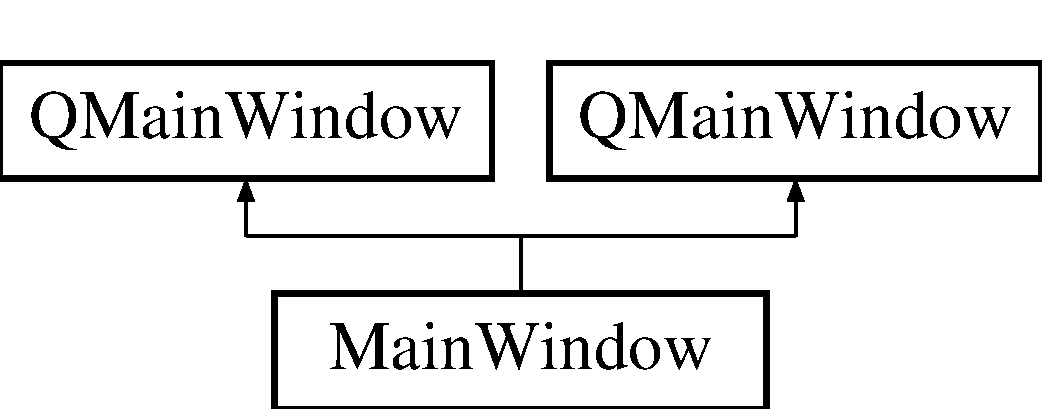
\includegraphics[height=2.000000cm]{classMainWindow}
\end{center}
\end{figure}
\subsection*{Public Member Functions}
\begin{DoxyCompactItemize}
\item 
\hypertarget{classMainWindow_a8b244be8b7b7db1b08de2a2acb9409db}{{\bfseries Main\-Window} (Q\-Widget $\ast$parent=0)}\label{classMainWindow_a8b244be8b7b7db1b08de2a2acb9409db}

\item 
\hypertarget{classMainWindow_a8b244be8b7b7db1b08de2a2acb9409db}{{\bfseries Main\-Window} (Q\-Widget $\ast$parent=0)}\label{classMainWindow_a8b244be8b7b7db1b08de2a2acb9409db}

\end{DoxyCompactItemize}
\subsection*{Protected Member Functions}
\begin{DoxyCompactItemize}
\item 
\hypertarget{classMainWindow_a2b5463ae209a03d1680b39c950dac8be}{void {\bfseries mouse\-Press\-Event} (Q\-Mouse\-Event $\ast$event)}\label{classMainWindow_a2b5463ae209a03d1680b39c950dac8be}

\item 
\hypertarget{classMainWindow_a2da19b23a75b83dcc8b8f6b6128463a3}{void {\bfseries paint\-Event} (Q\-Paint\-Event $\ast$)}\label{classMainWindow_a2da19b23a75b83dcc8b8f6b6128463a3}

\item 
\hypertarget{classMainWindow_a2b5463ae209a03d1680b39c950dac8be}{void {\bfseries mouse\-Press\-Event} (Q\-Mouse\-Event $\ast$event)}\label{classMainWindow_a2b5463ae209a03d1680b39c950dac8be}

\item 
\hypertarget{classMainWindow_a2da19b23a75b83dcc8b8f6b6128463a3}{void {\bfseries paint\-Event} (Q\-Paint\-Event $\ast$)}\label{classMainWindow_a2da19b23a75b83dcc8b8f6b6128463a3}

\end{DoxyCompactItemize}


\subsection{Detailed Description}


Definition at line 14 of file mainwindow.\-h.



The documentation for this class was generated from the following files\-:\begin{DoxyCompactItemize}
\item 
/home/michal/\-Desktop/aeris/src/map\-\_\-editor/mainwindow.\-h\item 
/home/michal/\-Desktop/aeris/src/map\-\_\-editor/mainwindow.\-cpp\end{DoxyCompactItemize}

\hypertarget{classUi_1_1MainWindow}{\section{Ui\-:\-:Main\-Window Class Reference}
\label{classUi_1_1MainWindow}\index{Ui\-::\-Main\-Window@{Ui\-::\-Main\-Window}}
}
Inheritance diagram for Ui\-:\-:Main\-Window\-:\begin{figure}[H]
\begin{center}
\leavevmode
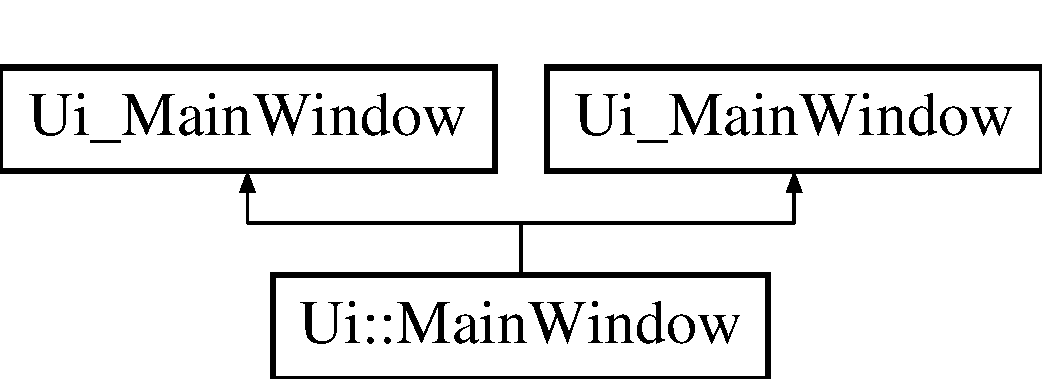
\includegraphics[height=2.000000cm]{classUi_1_1MainWindow}
\end{center}
\end{figure}
\subsection*{Additional Inherited Members}


\subsection{Detailed Description}


Definition at line 363 of file ui\-\_\-mainwindow.\-h.



The documentation for this class was generated from the following file\-:\begin{DoxyCompactItemize}
\item 
/home/michal/\-Desktop/aeris/src/map\-\_\-editor/ui\-\_\-mainwindow.\-h\end{DoxyCompactItemize}

\hypertarget{structqt__meta__stringdata__MainWindow__t}{\section{qt\-\_\-meta\-\_\-stringdata\-\_\-\-Main\-Window\-\_\-t Struct Reference}
\label{structqt__meta__stringdata__MainWindow__t}\index{qt\-\_\-meta\-\_\-stringdata\-\_\-\-Main\-Window\-\_\-t@{qt\-\_\-meta\-\_\-stringdata\-\_\-\-Main\-Window\-\_\-t}}
}
\subsection*{Public Attributes}
\begin{DoxyCompactItemize}
\item 
\hypertarget{structqt__meta__stringdata__MainWindow__t_a25333e8c3c2c62e1ac051146bc6c454f}{Q\-Byte\-Array\-Data {\bfseries data} \mbox{[}31\mbox{]}}\label{structqt__meta__stringdata__MainWindow__t_a25333e8c3c2c62e1ac051146bc6c454f}

\item 
\hypertarget{structqt__meta__stringdata__MainWindow__t_a9d3ed196ceaa4fc8c2e817fbeed3fea8}{char {\bfseries stringdata} \mbox{[}777\mbox{]}}\label{structqt__meta__stringdata__MainWindow__t_a9d3ed196ceaa4fc8c2e817fbeed3fea8}

\end{DoxyCompactItemize}


\subsection{Detailed Description}


Definition at line 21 of file moc\-\_\-mainwindow.\-cpp.



The documentation for this struct was generated from the following file\-:\begin{DoxyCompactItemize}
\item 
/home/michal/\-Desktop/aeris/src/map\-\_\-editor/moc\-\_\-mainwindow.\-cpp\end{DoxyCompactItemize}

\hypertarget{structsAction}{\section{s\-Action Struct Reference}
\label{structsAction}\index{s\-Action@{s\-Action}}
}
\subsection*{Public Attributes}
\begin{DoxyCompactItemize}
\item 
\hypertarget{structsAction_ab3037a9305dfc2c94d804c053a88bf9c}{float {\bfseries fitness}}\label{structsAction_ab3037a9305dfc2c94d804c053a88bf9c}

\item 
\hypertarget{structsAction_a04bcaa29a01f8fc26b6906ac3f584029}{std\-::vector$<$ float $>$ {\bfseries action}}\label{structsAction_a04bcaa29a01f8fc26b6906ac3f584029}

\end{DoxyCompactItemize}


\subsection{Detailed Description}


Definition at line 9 of file action.\-h.



The documentation for this struct was generated from the following file\-:\begin{DoxyCompactItemize}
\item 
/home/michal/\-Desktop/aeris/src/q\-\_\-learning/robot\-\_\-brain/action.\-h\end{DoxyCompactItemize}

\hypertarget{structsCFG}{\section{s\-C\-F\-G Struct Reference}
\label{structsCFG}\index{s\-C\-F\-G@{s\-C\-F\-G}}
}
\subsection*{Public Attributes}
\begin{DoxyCompactItemize}
\item 
\hypertarget{structsCFG_a5843faf50da251a07302ce4eee81e588}{u32 {\bfseries port}}\label{structsCFG_a5843faf50da251a07302ce4eee81e588}

\item 
\hypertarget{structsCFG_a97012388819824e5504e0e3c3d721cae}{u64 {\bfseries device\-\_\-id}}\label{structsCFG_a97012388819824e5504e0e3c3d721cae}

\item 
\hypertarget{structsCFG_afac8663ae031a58a4e13dcb0fd71d3cd}{char {\bfseries server\-\_\-name} \mbox{[}S\-E\-R\-V\-E\-R\-\_\-\-N\-A\-M\-E\-\_\-\-M\-A\-X\-\_\-\-L\-E\-N\-G\-T\-H+1\mbox{]}}\label{structsCFG_afac8663ae031a58a4e13dcb0fd71d3cd}

\end{DoxyCompactItemize}


\subsection{Detailed Description}


Definition at line 5 of file load\-\_\-cfg.\-cpp.



The documentation for this struct was generated from the following file\-:\begin{DoxyCompactItemize}
\item 
/home/michal/\-Desktop/aeris/src/virtual\-\_\-robot/0.\-0.\-7/common/load\-\_\-cfg.\-cpp\end{DoxyCompactItemize}

\hypertarget{structsDebugLog}{\section{s\-Debug\-Log Struct Reference}
\label{structsDebugLog}\index{s\-Debug\-Log@{s\-Debug\-Log}}
}
\subsection*{Public Attributes}
\begin{DoxyCompactItemize}
\item 
\hypertarget{structsDebugLog_a9241783d433fbe245355d7c802d256ca}{char {\bfseries file\-\_\-name} \mbox{[}F\-I\-L\-E\-N\-A\-M\-E\-\_\-\-M\-A\-X+1\mbox{]}}\label{structsDebugLog_a9241783d433fbe245355d7c802d256ca}

\item 
\hypertarget{structsDebugLog_a13963f4f51d07e60b0ded9d2931837a6}{F\-I\-L\-E $\ast$ {\bfseries fd}}\label{structsDebugLog_a13963f4f51d07e60b0ded9d2931837a6}

\item 
\hypertarget{structsDebugLog_adc7a9eff14d21090e2b4349bdd63072a}{pthread\-\_\-mutex\-\_\-t {\bfseries mutex}}\label{structsDebugLog_adc7a9eff14d21090e2b4349bdd63072a}

\end{DoxyCompactItemize}


\subsection{Detailed Description}


Definition at line 11 of file debug\-\_\-log.\-h.



The documentation for this struct was generated from the following file\-:\begin{DoxyCompactItemize}
\item 
/home/michal/\-Desktop/aeris/src/common/debug\-\_\-log.\-h\end{DoxyCompactItemize}

\hypertarget{structsMap}{\section{s\-Map Struct Reference}
\label{structsMap}\index{s\-Map@{s\-Map}}
}
\subsection*{Public Attributes}
\begin{DoxyCompactItemize}
\item 
\hypertarget{structsMap_a888fdd62c59aabd2acc042248f479ae5}{u32 {\bfseries magic}}\label{structsMap_a888fdd62c59aabd2acc042248f479ae5}

\item 
\hypertarget{structsMap_a699a06fb8a2cc41b06b06990c46488b3}{u32 {\bfseries type}}\label{structsMap_a699a06fb8a2cc41b06b06990c46488b3}

\item 
\hypertarget{structsMap_a04d056c46d281e64050a0bdf088e5306}{u32 {\bfseries id}}\label{structsMap_a04d056c46d281e64050a0bdf088e5306}

\item 
\hypertarget{structsMap_aad556c1771189cc0cf2a8fcb5807f7c0}{u32 {\bfseries width}}\label{structsMap_aad556c1771189cc0cf2a8fcb5807f7c0}

\item 
\hypertarget{structsMap_a91ad86a4b60aff6e96ead62f85bbb2df}{u32 {\bfseries height}}\label{structsMap_a91ad86a4b60aff6e96ead62f85bbb2df}

\item 
\hypertarget{structsMap_a1580fef54a11716cccf3aeec0e160158}{float {\bfseries base\-\_\-width}}\label{structsMap_a1580fef54a11716cccf3aeec0e160158}

\item 
\hypertarget{structsMap_a17a619b4cd27500646120fe430abf8af}{float {\bfseries base\-\_\-height}}\label{structsMap_a17a619b4cd27500646120fe430abf8af}

\item 
\hypertarget{structsMap_ab95fdcca6c5ff181dd89d1cacaa337d3}{struct \hyperlink{structsMapField}{s\-Map\-Field} $\ast$$\ast$ {\bfseries fields}}\label{structsMap_ab95fdcca6c5ff181dd89d1cacaa337d3}

\item 
\hypertarget{structsMap_a192a32e60d412fc6940a016fe22f6d9c}{void $\ast$ {\bfseries next\-\_\-info\-\_\-ptr}}\label{structsMap_a192a32e60d412fc6940a016fe22f6d9c}

\end{DoxyCompactItemize}


\subsection{Detailed Description}


Definition at line 46 of file map.\-h.



The documentation for this struct was generated from the following file\-:\begin{DoxyCompactItemize}
\item 
/home/michal/\-Desktop/aeris/src/common/map.\-h\end{DoxyCompactItemize}

\hypertarget{structsMapField}{\section{s\-Map\-Field Struct Reference}
\label{structsMapField}\index{s\-Map\-Field@{s\-Map\-Field}}
}
\subsection*{Public Attributes}
\begin{DoxyCompactItemize}
\item 
\hypertarget{structsMapField_aeced840714c5559d2df1da458e1a4cd0}{u32 {\bfseries type}}\label{structsMapField_aeced840714c5559d2df1da458e1a4cd0}

\item 
\hypertarget{structsMapField_a8900aa98020edb668ad7adf2ff65a4d6}{u32 {\bfseries id}}\label{structsMapField_a8900aa98020edb668ad7adf2ff65a4d6}

\item 
\hypertarget{structsMapField_a979c036f4bc3a63667dab8eb101ae578}{u32 {\bfseries texture\-\_\-id}}\label{structsMapField_a979c036f4bc3a63667dab8eb101ae578}

\item 
\hypertarget{structsMapField_ad01d29cde28c22771a2a7810ae255c5c}{i32 {\bfseries parameter\-\_\-int}}\label{structsMapField_ad01d29cde28c22771a2a7810ae255c5c}

\item 
\hypertarget{structsMapField_a93b5280433256a0564226f7289e0afaf}{float {\bfseries parameter\-\_\-f}}\label{structsMapField_a93b5280433256a0564226f7289e0afaf}

\item 
\hypertarget{structsMapField_aa6e68c3d07bff370d335b7d0c34e41ab}{float {\bfseries reward}}\label{structsMapField_aa6e68c3d07bff370d335b7d0c34e41ab}

\item 
\hypertarget{structsMapField_ae8a51917bd125b1ded83536f5ac62b6f}{float {\bfseries position} \mbox{[}4\mbox{]}}\label{structsMapField_ae8a51917bd125b1ded83536f5ac62b6f}

\item 
\hypertarget{structsMapField_a70c6292d2c2581cce7487a9586d39173}{float {\bfseries color} \mbox{[}4\mbox{]}}\label{structsMapField_a70c6292d2c2581cce7487a9586d39173}

\item 
\hypertarget{structsMapField_a244dedc5792cf5bf6613e91d1dced91b}{void $\ast$ {\bfseries next\-\_\-info\-\_\-ptr}}\label{structsMapField_a244dedc5792cf5bf6613e91d1dced91b}

\end{DoxyCompactItemize}


\subsection{Detailed Description}


Definition at line 29 of file map.\-h.



The documentation for this struct was generated from the following file\-:\begin{DoxyCompactItemize}
\item 
/home/michal/\-Desktop/aeris/src/common/map.\-h\end{DoxyCompactItemize}

\hypertarget{structsNeuralNetwork}{\section{s\-Neural\-Network Struct Reference}
\label{structsNeuralNetwork}\index{s\-Neural\-Network@{s\-Neural\-Network}}
}
\subsection*{Public Attributes}
\begin{DoxyCompactItemize}
\item 
\hypertarget{structsNeuralNetwork_ae70c71dabeb927ba5e375208bd6e9a66}{u32 {\bfseries layers\-\_\-count}}\label{structsNeuralNetwork_ae70c71dabeb927ba5e375208bd6e9a66}

\item 
\hypertarget{structsNeuralNetwork_aa425ee3d56e13661dce5f34c479f798c}{u32 {\bfseries order}}\label{structsNeuralNetwork_aa425ee3d56e13661dce5f34c479f798c}

\item 
\hypertarget{structsNeuralNetwork_a227c146a256519503657c80790cf11a5}{u32 $\ast$ {\bfseries size\-\_\-input}}\label{structsNeuralNetwork_a227c146a256519503657c80790cf11a5}

\item 
\hypertarget{structsNeuralNetwork_a429a03c98bb824fb2bdcd7649376741e}{u32 $\ast$ {\bfseries size\-\_\-input\-\_\-}}\label{structsNeuralNetwork_a429a03c98bb824fb2bdcd7649376741e}

\item 
\hypertarget{structsNeuralNetwork_ae383e858cd9d9361410d88d5004528c6}{u32 $\ast$ {\bfseries size\-\_\-output}}\label{structsNeuralNetwork_ae383e858cd9d9361410d88d5004528c6}

\item 
\hypertarget{structsNeuralNetwork_a81f438dae1a676730e3b99643ea4a3e6}{float {\bfseries learning\-\_\-constant}}\label{structsNeuralNetwork_a81f438dae1a676730e3b99643ea4a3e6}

\item 
\hypertarget{structsNeuralNetwork_aff7a0e1da9e3b24efb8d3e6d6df3713b}{float {\bfseries weight\-\_\-range}}\label{structsNeuralNetwork_aff7a0e1da9e3b24efb8d3e6d6df3713b}

\item 
\hypertarget{structsNeuralNetwork_ad5d72b18f56aec7bdbc1c837b57e8487}{float $\ast$$\ast$$\ast$ {\bfseries w}}\label{structsNeuralNetwork_ad5d72b18f56aec7bdbc1c837b57e8487}

\item 
\hypertarget{structsNeuralNetwork_ad67a1b3c839c54b84e124c8fe2833139}{float $\ast$$\ast$ {\bfseries output}}\label{structsNeuralNetwork_ad67a1b3c839c54b84e124c8fe2833139}

\item 
\hypertarget{structsNeuralNetwork_a460d9fac83d0bcd64f9cd7aa5a84c591}{float $\ast$$\ast$ {\bfseries error}}\label{structsNeuralNetwork_a460d9fac83d0bcd64f9cd7aa5a84c591}

\item 
\hypertarget{structsNeuralNetwork_afef1fcb46cc11082d1f872f1326fafcb}{float $\ast$$\ast$ {\bfseries input}}\label{structsNeuralNetwork_afef1fcb46cc11082d1f872f1326fafcb}

\item 
\hypertarget{structsNeuralNetwork_af7c1f10e277310626387499c80917fcd}{float $\ast$$\ast$ {\bfseries input\-\_\-}}\label{structsNeuralNetwork_af7c1f10e277310626387499c80917fcd}

\end{DoxyCompactItemize}


\subsection{Detailed Description}


Definition at line 16 of file neural\-\_\-network.\-h.



The documentation for this struct was generated from the following file\-:\begin{DoxyCompactItemize}
\item 
/home/michal/\-Desktop/aeris/src/virtual\-\_\-robot/0.\-0.\-7/common/robot/neural\-\_\-network/neural\-\_\-network.\-h\end{DoxyCompactItemize}

\hypertarget{structsNeuralNetworkInitStructure}{\section{s\-Neural\-Network\-Init\-Structure Struct Reference}
\label{structsNeuralNetworkInitStructure}\index{s\-Neural\-Network\-Init\-Structure@{s\-Neural\-Network\-Init\-Structure}}
}
\subsection*{Public Attributes}
\begin{DoxyCompactItemize}
\item 
\hypertarget{structsNeuralNetworkInitStructure_a1631b065b3e498501560fc01459e5cd6}{u32 {\bfseries init\-\_\-vector\-\_\-size}}\label{structsNeuralNetworkInitStructure_a1631b065b3e498501560fc01459e5cd6}

\item 
\hypertarget{structsNeuralNetworkInitStructure_af304870dfad5e2edd63d65e07823277b}{u32 $\ast$ {\bfseries init\-\_\-vector}}\label{structsNeuralNetworkInitStructure_af304870dfad5e2edd63d65e07823277b}

\item 
\hypertarget{structsNeuralNetworkInitStructure_a178a18e0fbce1fde7aee0a573ca73844}{float {\bfseries weight\-\_\-range}}\label{structsNeuralNetworkInitStructure_a178a18e0fbce1fde7aee0a573ca73844}

\item 
\hypertarget{structsNeuralNetworkInitStructure_a711d79f75658f78332439172b5d1d218}{float {\bfseries learning\-\_\-constant}}\label{structsNeuralNetworkInitStructure_a711d79f75658f78332439172b5d1d218}

\item 
\hypertarget{structsNeuralNetworkInitStructure_a1d256740ebce6dd49c27c7f24f227ffa}{u32 {\bfseries order}}\label{structsNeuralNetworkInitStructure_a1d256740ebce6dd49c27c7f24f227ffa}

\item 
\hypertarget{structsNeuralNetworkInitStructure_a73c705e844c05b2ca59a42a77e52e130}{u32 {\bfseries neuron\-\_\-type}}\label{structsNeuralNetworkInitStructure_a73c705e844c05b2ca59a42a77e52e130}

\end{DoxyCompactItemize}


\subsection{Detailed Description}


Definition at line 6 of file neural\-\_\-network.\-h.



The documentation for this struct was generated from the following file\-:\begin{DoxyCompactItemize}
\item 
/home/michal/\-Desktop/aeris/src/virtual\-\_\-robot/0.\-0.\-7/common/robot/neural\-\_\-network/neural\-\_\-network.\-h\end{DoxyCompactItemize}

\hypertarget{structsNNLayer}{\section{s\-N\-N\-Layer Struct Reference}
\label{structsNNLayer}\index{s\-N\-N\-Layer@{s\-N\-N\-Layer}}
}
\subsection*{Public Attributes}
\begin{DoxyCompactItemize}
\item 
\hypertarget{structsNNLayer_a39671ebb687538cad1faa9f4f2fb56f8}{u32 {\bfseries input\-\_\-size}}\label{structsNNLayer_a39671ebb687538cad1faa9f4f2fb56f8}

\item 
\hypertarget{structsNNLayer_ac7b939bb9db7f36934bb1bf4c98d4cf3}{u32 {\bfseries \-\_\-input\-\_\-size}}\label{structsNNLayer_ac7b939bb9db7f36934bb1bf4c98d4cf3}

\item 
\hypertarget{structsNNLayer_aa0e6b38d5cdb5472c2a6fd38ba3cce61}{u32 {\bfseries output\-\_\-size}}\label{structsNNLayer_aa0e6b38d5cdb5472c2a6fd38ba3cce61}

\item 
\hypertarget{structsNNLayer_a2786af56ba6dd2cdb1c6b41dee628c3f}{u32 {\bfseries order}}\label{structsNNLayer_a2786af56ba6dd2cdb1c6b41dee628c3f}

\item 
\hypertarget{structsNNLayer_a6615b9379c48cff23c0fc7bc92614252}{float $\ast$ {\bfseries input}}\label{structsNNLayer_a6615b9379c48cff23c0fc7bc92614252}

\item 
\hypertarget{structsNNLayer_aefbe1fdae7c6c78988da5ec1de5aa748}{float $\ast$ {\bfseries \-\_\-input}}\label{structsNNLayer_aefbe1fdae7c6c78988da5ec1de5aa748}

\item 
\hypertarget{structsNNLayer_aa16baf629e32b388f4798f7a381e8edf}{float $\ast$$\ast$ {\bfseries w}}\label{structsNNLayer_aa16baf629e32b388f4798f7a381e8edf}

\item 
\hypertarget{structsNNLayer_aaf74d7dc9c777358051ade70be8354bb}{float $\ast$ {\bfseries output}}\label{structsNNLayer_aaf74d7dc9c777358051ade70be8354bb}

\item 
\hypertarget{structsNNLayer_a1350a2df8b3030aace58189145c154ff}{float $\ast$ {\bfseries error}}\label{structsNNLayer_a1350a2df8b3030aace58189145c154ff}

\item 
\hypertarget{structsNNLayer_affeefed95f5500cb10678b0ab91fcf61}{float {\bfseries weight\-\_\-range}}\label{structsNNLayer_affeefed95f5500cb10678b0ab91fcf61}

\item 
\hypertarget{structsNNLayer_abb9e00388cf8220ce986ce82b934d40c}{u32 {\bfseries neuron\-\_\-type}}\label{structsNNLayer_abb9e00388cf8220ce986ce82b934d40c}

\end{DoxyCompactItemize}


\subsection{Detailed Description}


Definition at line 6 of file nn.\-h.



The documentation for this struct was generated from the following file\-:\begin{DoxyCompactItemize}
\item 
/home/michal/\-Desktop/aeris/src/virtual\-\_\-robot/0.\-0.\-7/common/robot/neural\-\_\-network/nn.\-h\end{DoxyCompactItemize}

\hypertarget{structsPoint3D}{\section{s\-Point3\-D Struct Reference}
\label{structsPoint3D}\index{s\-Point3\-D@{s\-Point3\-D}}
}
\subsection*{Public Attributes}
\begin{DoxyCompactItemize}
\item 
\hypertarget{structsPoint3D_acd4c193396e478aa3c9b7c4c70849036}{float {\bfseries x}}\label{structsPoint3D_acd4c193396e478aa3c9b7c4c70849036}

\item 
\hypertarget{structsPoint3D_a234675cf0d8e2c4dd9673e6f6053d6a1}{float {\bfseries y}}\label{structsPoint3D_a234675cf0d8e2c4dd9673e6f6053d6a1}

\item 
\hypertarget{structsPoint3D_a2a0b8b20e1f52897edaba1c100bcc194}{float {\bfseries z}}\label{structsPoint3D_a2a0b8b20e1f52897edaba1c100bcc194}

\item 
\hypertarget{structsPoint3D_a0a8e9058df01aa712857f7d16f9b6aa0}{float {\bfseries r}}\label{structsPoint3D_a0a8e9058df01aa712857f7d16f9b6aa0}

\item 
\hypertarget{structsPoint3D_a1610fae258ff1dcb06c5c502443a6898}{float {\bfseries g}}\label{structsPoint3D_a1610fae258ff1dcb06c5c502443a6898}

\item 
\hypertarget{structsPoint3D_a79f80d6cc4aff90b3512d52aa8bafc45}{float {\bfseries b}}\label{structsPoint3D_a79f80d6cc4aff90b3512d52aa8bafc45}

\end{DoxyCompactItemize}


\subsection{Detailed Description}


Definition at line 15 of file math.\-h.



The documentation for this struct was generated from the following file\-:\begin{DoxyCompactItemize}
\item 
/home/michal/\-Desktop/aeris/src/common/math.\-h\end{DoxyCompactItemize}

\hypertarget{structsRobot}{\section{s\-Robot Struct Reference}
\label{structsRobot}\index{s\-Robot@{s\-Robot}}
}
\subsection*{Public Attributes}
\begin{DoxyCompactItemize}
\item 
\hypertarget{structsRobot_acf6d1a5a8d9024cbe6efcd5c5b421916}{u64 {\bfseries id}}\label{structsRobot_acf6d1a5a8d9024cbe6efcd5c5b421916}

\item 
\hypertarget{structsRobot_afc0670f677fc59982378f53f3cecefe4}{u32 {\bfseries type}}\label{structsRobot_afc0670f677fc59982378f53f3cecefe4}

\item 
\hypertarget{structsRobot_ab6f3d5c45c246e0d8b46a31cf94338a3}{u32 {\bfseries request}}\label{structsRobot_ab6f3d5c45c246e0d8b46a31cf94338a3}

\item 
\hypertarget{structsRobot_ac1c416ef8f2316726f3b835fb06f2474}{u32 {\bfseries parameter}}\label{structsRobot_ac1c416ef8f2316726f3b835fb06f2474}

\item 
\hypertarget{structsRobot_adb204dd2d289ebab8178309ae815ac47}{float {\bfseries d} \mbox{[}R\-O\-B\-O\-T\-\_\-\-S\-P\-A\-C\-E\-\_\-\-D\-I\-M\-E\-N\-S\-I\-O\-N\mbox{]}}\label{structsRobot_adb204dd2d289ebab8178309ae815ac47}

\item 
\hypertarget{structsRobot_a723c6e8327be50f8f7edf5894f11fba2}{float {\bfseries position} \mbox{[}R\-O\-B\-O\-T\-\_\-\-S\-P\-A\-C\-E\-\_\-\-D\-I\-M\-E\-N\-S\-I\-O\-N\mbox{]}}\label{structsRobot_a723c6e8327be50f8f7edf5894f11fba2}

\item 
\hypertarget{structsRobot_a044ce4ac3802a9f99da743b7d85556ab}{float {\bfseries sensors} \mbox{[}R\-O\-B\-O\-T\-\_\-\-S\-E\-N\-S\-O\-R\-S\-\_\-\-C\-O\-U\-N\-T\mbox{]}}\label{structsRobot_a044ce4ac3802a9f99da743b7d85556ab}

\item 
\hypertarget{structsRobot_a7ef86a7202a493cdf4aa3ada4ba6bb73}{float {\bfseries angles} \mbox{[}R\-O\-B\-O\-T\-\_\-\-S\-P\-A\-C\-E\-\_\-\-D\-I\-M\-E\-N\-S\-I\-O\-N\mbox{]}}\label{structsRobot_a7ef86a7202a493cdf4aa3ada4ba6bb73}

\item 
\hypertarget{structsRobot_a8372b40f963ae1b085f475c88db6b95d}{float {\bfseries dt}}\label{structsRobot_a8372b40f963ae1b085f475c88db6b95d}

\item 
\hypertarget{structsRobot_aa052d09b89c7a23910fbb182eb83c1f9}{double {\bfseries time}}\label{structsRobot_aa052d09b89c7a23910fbb182eb83c1f9}

\item 
\hypertarget{structsRobot_a41c5367091185062b6c0427bea68e8fe}{i32 {\bfseries parameter\-\_\-int}}\label{structsRobot_a41c5367091185062b6c0427bea68e8fe}

\item 
\hypertarget{structsRobot_a0398e11d41ff96b5893e7a2483792c4b}{float {\bfseries parameter\-\_\-f}}\label{structsRobot_a0398e11d41ff96b5893e7a2483792c4b}

\item 
\hypertarget{structsRobot_a407e2628f2abc97ec7ac6470bdbd3d6f}{float {\bfseries reward}}\label{structsRobot_a407e2628f2abc97ec7ac6470bdbd3d6f}

\item 
\hypertarget{structsRobot_ad727fed7aeb4e6269ca956c06dc78df0}{float {\bfseries colision\-\_\-distance}}\label{structsRobot_ad727fed7aeb4e6269ca956c06dc78df0}

\end{DoxyCompactItemize}


\subsection{Detailed Description}


Definition at line 29 of file s\-\_\-robot.\-h.



The documentation for this struct was generated from the following file\-:\begin{DoxyCompactItemize}
\item 
/home/michal/\-Desktop/aeris/src/virtual\-\_\-robot/0.\-0.\-7/common/robot/s\-\_\-robot.\-h\end{DoxyCompactItemize}

\hypertarget{structsRobotInitStruct}{\section{s\-Robot\-Init\-Struct Struct Reference}
\label{structsRobotInitStruct}\index{s\-Robot\-Init\-Struct@{s\-Robot\-Init\-Struct}}
}
\subsection*{Public Attributes}
\begin{DoxyCompactItemize}
\item 
\hypertarget{structsRobotInitStruct_a05e89c42a36672d311f9b55450feae7e}{u32 {\bfseries inputs\-\_\-count}}\label{structsRobotInitStruct_a05e89c42a36672d311f9b55450feae7e}

\item 
\hypertarget{structsRobotInitStruct_a839c496b7223fee6a6e05ecb30fd8479}{u32 {\bfseries outputs\-\_\-count}}\label{structsRobotInitStruct_a839c496b7223fee6a6e05ecb30fd8479}

\item 
\hypertarget{structsRobotInitStruct_ae623fe7ed544e62fc890c49d2034a16d}{u32 {\bfseries actions\-\_\-per\-\_\-state}}\label{structsRobotInitStruct_ae623fe7ed544e62fc890c49d2034a16d}

\item 
\hypertarget{structsRobotInitStruct_aa1330020b05390b0bbf520beb295b66e}{u32 {\bfseries states\-\_\-count}}\label{structsRobotInitStruct_aa1330020b05390b0bbf520beb295b66e}

\item 
\hypertarget{structsRobotInitStruct_a9e0c80bff990a6831a763c05566e50f3}{u32 {\bfseries type}}\label{structsRobotInitStruct_a9e0c80bff990a6831a763c05566e50f3}

\item 
\hypertarget{structsRobotInitStruct_aa8d35d148e84132ce6474d2c457df3f8}{u32 {\bfseries path\-\_\-max\-\_\-length}}\label{structsRobotInitStruct_aa8d35d148e84132ce6474d2c457df3f8}

\item 
\hypertarget{structsRobotInitStruct_ad4b7c744480abad13b31f5e61a62ce81}{std\-::vector$<$ float $>$ {\bfseries position\-\_\-max}}\label{structsRobotInitStruct_ad4b7c744480abad13b31f5e61a62ce81}

\end{DoxyCompactItemize}


\subsection{Detailed Description}


Definition at line 8 of file robot.\-h.



The documentation for this struct was generated from the following files\-:\begin{DoxyCompactItemize}
\item 
/home/michal/\-Desktop/aeris/src/q\-\_\-learning/robot\-\_\-brain/robot.\-h\item 
/home/michal/\-Desktop/aeris/src/q\-\_\-learning/robot\-\_\-brain/robot.\-h$\sim$\end{DoxyCompactItemize}

\hypertarget{structsSquare}{\section{s\-Square Struct Reference}
\label{structsSquare}\index{s\-Square@{s\-Square}}
}
\subsection*{Public Attributes}
\begin{DoxyCompactItemize}
\item 
\hypertarget{structsSquare_a4a2dd9356d4cb1acbf86f030b89822d9}{float {\bfseries x}}\label{structsSquare_a4a2dd9356d4cb1acbf86f030b89822d9}

\item 
\hypertarget{structsSquare_a2fa7edb394b6c87ded17a1ee2c5068b5}{float {\bfseries y}}\label{structsSquare_a2fa7edb394b6c87ded17a1ee2c5068b5}

\item 
\hypertarget{structsSquare_aab96ddab543d8c6d1c93a83f6644c848}{float {\bfseries z}}\label{structsSquare_aab96ddab543d8c6d1c93a83f6644c848}

\item 
\hypertarget{structsSquare_a31b3d5a3a4c151737daf309844daf5fa}{float {\bfseries r}}\label{structsSquare_a31b3d5a3a4c151737daf309844daf5fa}

\item 
\hypertarget{structsSquare_a2b9691ec7db5c116addab6b6f970fb39}{float {\bfseries g}}\label{structsSquare_a2b9691ec7db5c116addab6b6f970fb39}

\item 
\hypertarget{structsSquare_a901968400d6dec96e332e75017951d05}{float {\bfseries b}}\label{structsSquare_a901968400d6dec96e332e75017951d05}

\item 
\hypertarget{structsSquare_a3830c43662fe9362d3df4f7106a6b560}{float {\bfseries x\-\_\-size}}\label{structsSquare_a3830c43662fe9362d3df4f7106a6b560}

\item 
\hypertarget{structsSquare_a3c5c8e92e1884d361d33fc2818177f21}{float {\bfseries y\-\_\-size}}\label{structsSquare_a3c5c8e92e1884d361d33fc2818177f21}

\item 
\hypertarget{structsSquare_a6ddcb8b967bb21ab54f3eb2cd16d198b}{float {\bfseries z\-\_\-size}}\label{structsSquare_a6ddcb8b967bb21ab54f3eb2cd16d198b}

\end{DoxyCompactItemize}


\subsection{Detailed Description}


Definition at line 9 of file app\-\_\-core.\-h.



The documentation for this struct was generated from the following file\-:\begin{DoxyCompactItemize}
\item 
/home/michal/\-Desktop/aeris/src/map\-\_\-editor/app\-\_\-core.\-h\end{DoxyCompactItemize}

\hypertarget{structsVect3D}{\section{s\-Vect3\-D Struct Reference}
\label{structsVect3D}\index{s\-Vect3\-D@{s\-Vect3\-D}}
}
\subsection*{Public Attributes}
\begin{DoxyCompactItemize}
\item 
\hypertarget{structsVect3D_a23b2575c1306f5030047684cb32e69f1}{float {\bfseries x}}\label{structsVect3D_a23b2575c1306f5030047684cb32e69f1}

\item 
\hypertarget{structsVect3D_a06685dd96cf77950ab98e19bc7760e96}{float {\bfseries y}}\label{structsVect3D_a06685dd96cf77950ab98e19bc7760e96}

\item 
\hypertarget{structsVect3D_a66ee454bab8eb16c0b521feea05fc51b}{float {\bfseries z}}\label{structsVect3D_a66ee454bab8eb16c0b521feea05fc51b}

\end{DoxyCompactItemize}


\subsection{Detailed Description}


Definition at line 10 of file math.\-h.



The documentation for this struct was generated from the following file\-:\begin{DoxyCompactItemize}
\item 
/home/michal/\-Desktop/aeris/src/common/math.\-h\end{DoxyCompactItemize}

\hypertarget{structsVector}{\section{s\-Vector Struct Reference}
\label{structsVector}\index{s\-Vector@{s\-Vector}}
}
\subsection*{Public Attributes}
\begin{DoxyCompactItemize}
\item 
\hypertarget{structsVector_a4709eee0b2ac996456a703e2110afa99}{float $\ast$ {\bfseries points}}\label{structsVector_a4709eee0b2ac996456a703e2110afa99}

\item 
\hypertarget{structsVector_adc9ef8c0eed8f015533a62f9ff542381}{u32 {\bfseries size}}\label{structsVector_adc9ef8c0eed8f015533a62f9ff542381}

\end{DoxyCompactItemize}


\subsection{Detailed Description}


Definition at line 21 of file math.\-h.



The documentation for this struct was generated from the following file\-:\begin{DoxyCompactItemize}
\item 
/home/michal/\-Desktop/aeris/src/common/math.\-h\end{DoxyCompactItemize}

\hypertarget{structsVisualisation}{\section{s\-Visualisation Struct Reference}
\label{structsVisualisation}\index{s\-Visualisation@{s\-Visualisation}}
}
\subsection*{Public Attributes}
\begin{DoxyCompactItemize}
\item 
\hypertarget{structsVisualisation_a6f55371d0dfae2930c841caf63d606d7}{i32 {\bfseries window\-\_\-width}}\label{structsVisualisation_a6f55371d0dfae2930c841caf63d606d7}

\item 
\hypertarget{structsVisualisation_acc598e42a411c05bee4b9aed5b954790}{i32 {\bfseries window\-\_\-height}}\label{structsVisualisation_acc598e42a411c05bee4b9aed5b954790}

\item 
\hypertarget{structsVisualisation_aba3c48c2141ed751aef9481c12e7f11f}{float {\bfseries size}}\label{structsVisualisation_aba3c48c2141ed751aef9481c12e7f11f}

\item 
\hypertarget{structsVisualisation_a86342946290bdea4016c472fbc5bf2ea}{float {\bfseries angle}}\label{structsVisualisation_a86342946290bdea4016c472fbc5bf2ea}

\item 
\hypertarget{structsVisualisation_a32b06d36bc76f1f7a564add09c7598e9}{float {\bfseries ratio}}\label{structsVisualisation_a32b06d36bc76f1f7a564add09c7598e9}

\item 
\hypertarget{structsVisualisation_a93c5229f0e57f612ea1cf3cfbbac9386}{float {\bfseries position\-\_\-max\-\_\-x}}\label{structsVisualisation_a93c5229f0e57f612ea1cf3cfbbac9386}

\item 
\hypertarget{structsVisualisation_ace3bcfe425f13bed7352c448a4f1632d}{float {\bfseries position\-\_\-max\-\_\-y}}\label{structsVisualisation_ace3bcfe425f13bed7352c448a4f1632d}

\item 
\hypertarget{structsVisualisation_a99a98da3ed938821805edece74c8c72c}{float {\bfseries position\-\_\-max\-\_\-z}}\label{structsVisualisation_a99a98da3ed938821805edece74c8c72c}

\item 
\hypertarget{structsVisualisation_ae3289ed01b623a58dd6bbad98a925dcb}{u32 {\bfseries view\-\_\-state}}\label{structsVisualisation_ae3289ed01b623a58dd6bbad98a925dcb}

\item 
\hypertarget{structsVisualisation_aac9a3bc6ab4c53dedc41f3f389c77663}{std\-::thread $\ast$ {\bfseries rendering\-\_\-thread\-\_\-main\-\_\-loop}}\label{structsVisualisation_aac9a3bc6ab4c53dedc41f3f389c77663}

\item 
\hypertarget{structsVisualisation_a6d9ac505605739c8d689ac106457c056}{std\-::vector$<$ struct \hyperlink{structsRobot}{s\-Robot} $>$ {\bfseries robots}}\label{structsVisualisation_a6d9ac505605739c8d689ac106457c056}

\item 
\hypertarget{structsVisualisation_ae334065d927faa181d4ca4559aba2fa3}{std\-::mutex {\bfseries mutex}}\label{structsVisualisation_ae334065d927faa181d4ca4559aba2fa3}

\item 
\hypertarget{structsVisualisation_a02f4f8550fb3868e704829218a5219e3}{float {\bfseries base\-\_\-size}}\label{structsVisualisation_a02f4f8550fb3868e704829218a5219e3}

\end{DoxyCompactItemize}


\subsection{Detailed Description}


Definition at line 16 of file visualisation\-\_\-gl.\-h.



The documentation for this struct was generated from the following file\-:\begin{DoxyCompactItemize}
\item 
/home/michal/\-Desktop/aeris/src/virtual\-\_\-robot/0.\-0.\-7/common/visualisation\-\_\-gl.\-h\end{DoxyCompactItemize}

\hypertarget{classUi__MainWindow}{\section{Ui\-\_\-\-Main\-Window Class Reference}
\label{classUi__MainWindow}\index{Ui\-\_\-\-Main\-Window@{Ui\-\_\-\-Main\-Window}}
}
Inheritance diagram for Ui\-\_\-\-Main\-Window\-:\begin{figure}[H]
\begin{center}
\leavevmode
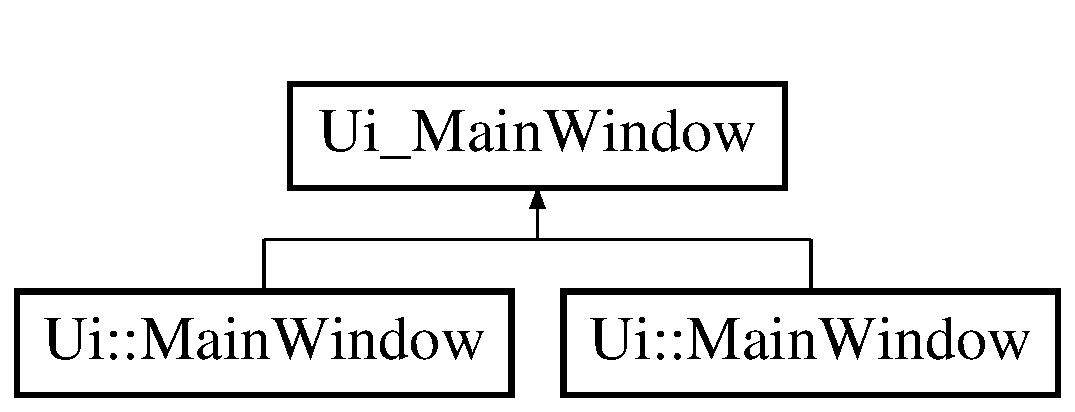
\includegraphics[height=2.000000cm]{classUi__MainWindow}
\end{center}
\end{figure}
\subsection*{Public Member Functions}
\begin{DoxyCompactItemize}
\item 
\hypertarget{classUi__MainWindow_acf4a0872c4c77d8f43a2ec66ed849b58}{void {\bfseries setup\-Ui} (Q\-Main\-Window $\ast$\hyperlink{classMainWindow}{Main\-Window})}\label{classUi__MainWindow_acf4a0872c4c77d8f43a2ec66ed849b58}

\item 
\hypertarget{classUi__MainWindow_a097dd160c3534a204904cb374412c618}{void {\bfseries retranslate\-Ui} (Q\-Main\-Window $\ast$\hyperlink{classMainWindow}{Main\-Window})}\label{classUi__MainWindow_a097dd160c3534a204904cb374412c618}

\item 
\hypertarget{classUi__MainWindow_acf4a0872c4c77d8f43a2ec66ed849b58}{void {\bfseries setup\-Ui} (Q\-Main\-Window $\ast$\hyperlink{classMainWindow}{Main\-Window})}\label{classUi__MainWindow_acf4a0872c4c77d8f43a2ec66ed849b58}

\item 
\hypertarget{classUi__MainWindow_a097dd160c3534a204904cb374412c618}{void {\bfseries retranslate\-Ui} (Q\-Main\-Window $\ast$\hyperlink{classMainWindow}{Main\-Window})}\label{classUi__MainWindow_a097dd160c3534a204904cb374412c618}

\end{DoxyCompactItemize}
\subsection*{Public Attributes}
\begin{DoxyCompactItemize}
\item 
\hypertarget{classUi__MainWindow_a6a80a45759b1781610e10b9cce031467}{Q\-Action $\ast$ {\bfseries action\-Open}}\label{classUi__MainWindow_a6a80a45759b1781610e10b9cce031467}

\item 
\hypertarget{classUi__MainWindow_a500c9596c58bca9e02263cbadf04a8e9}{Q\-Action $\ast$ {\bfseries action\-Save}}\label{classUi__MainWindow_a500c9596c58bca9e02263cbadf04a8e9}

\item 
\hypertarget{classUi__MainWindow_aa0efb782b40f398fb9fe6a7e2c59df20}{Q\-Action $\ast$ {\bfseries action\-Save\-\_\-as}}\label{classUi__MainWindow_aa0efb782b40f398fb9fe6a7e2c59df20}

\item 
\hypertarget{classUi__MainWindow_a38fb3262bc0ae2af350b689681b37379}{Q\-Action $\ast$ {\bfseries action\-Close}}\label{classUi__MainWindow_a38fb3262bc0ae2af350b689681b37379}

\item 
\hypertarget{classUi__MainWindow_a2c7ea4bcfe050588e76afd5c4dd61430}{Q\-Action $\ast$ {\bfseries action\-Delete}}\label{classUi__MainWindow_a2c7ea4bcfe050588e76afd5c4dd61430}

\item 
\hypertarget{classUi__MainWindow_a3dfc05dca8af14b1770d63afc9991c47}{Q\-Action $\ast$ {\bfseries action\-Wall}}\label{classUi__MainWindow_a3dfc05dca8af14b1770d63afc9991c47}

\item 
\hypertarget{classUi__MainWindow_a709dd8b518fd213177e241f114acfc18}{Q\-Action $\ast$ {\bfseries action\-Red\-\_\-robot}}\label{classUi__MainWindow_a709dd8b518fd213177e241f114acfc18}

\item 
\hypertarget{classUi__MainWindow_ab8e887d432e7efda61bb8dc12a7229dc}{Q\-Action $\ast$ {\bfseries action\-Red\-\_\-target}}\label{classUi__MainWindow_ab8e887d432e7efda61bb8dc12a7229dc}

\item 
\hypertarget{classUi__MainWindow_a72a7c77fa9e9967e028b8357c741a301}{Q\-Action $\ast$ {\bfseries action\-Red\-\_\-path}}\label{classUi__MainWindow_a72a7c77fa9e9967e028b8357c741a301}

\item 
\hypertarget{classUi__MainWindow_accfd5a3984afc55381398d7d3d6a159d}{Q\-Action $\ast$ {\bfseries action\-Green\-\_\-robot}}\label{classUi__MainWindow_accfd5a3984afc55381398d7d3d6a159d}

\item 
\hypertarget{classUi__MainWindow_a37a8de585e95065c82229645908cbfa8}{Q\-Action $\ast$ {\bfseries action\-Green\-\_\-target}}\label{classUi__MainWindow_a37a8de585e95065c82229645908cbfa8}

\item 
\hypertarget{classUi__MainWindow_abc40086804b67e4842e13a02e869a6d3}{Q\-Action $\ast$ {\bfseries action\-Green\-\_\-path}}\label{classUi__MainWindow_abc40086804b67e4842e13a02e869a6d3}

\item 
\hypertarget{classUi__MainWindow_adacffe9ce99ded0903006f64bbe24bdc}{Q\-Action $\ast$ {\bfseries action\-Blue\-\_\-robot}}\label{classUi__MainWindow_adacffe9ce99ded0903006f64bbe24bdc}

\item 
\hypertarget{classUi__MainWindow_aa5b5b2e6e20fbf3e0677a795f512724f}{Q\-Action $\ast$ {\bfseries action\-Blue\-\_\-target}}\label{classUi__MainWindow_aa5b5b2e6e20fbf3e0677a795f512724f}

\item 
\hypertarget{classUi__MainWindow_aa1e816d276964dc2832812482b7c60b3}{Q\-Action $\ast$ {\bfseries action\-Blue\-\_\-path}}\label{classUi__MainWindow_aa1e816d276964dc2832812482b7c60b3}

\item 
\hypertarget{classUi__MainWindow_a75a1fa9476f503f9bb8ca766a54005d0}{Q\-Action $\ast$ {\bfseries action\-Path}}\label{classUi__MainWindow_a75a1fa9476f503f9bb8ca766a54005d0}

\item 
\hypertarget{classUi__MainWindow_a93819e9dad932142e9de72e30e95e15a}{Q\-Action $\ast$ {\bfseries action\-Target}}\label{classUi__MainWindow_a93819e9dad932142e9de72e30e95e15a}

\item 
\hypertarget{classUi__MainWindow_ac49e795f421b857ba9a34c78f34c925a}{Q\-Action $\ast$ {\bfseries action\-Source}}\label{classUi__MainWindow_ac49e795f421b857ba9a34c78f34c925a}

\item 
\hypertarget{classUi__MainWindow_ad09b18bcae1d501c5f6ef66926e6b1bc}{Q\-Action $\ast$ {\bfseries action\-Destination}}\label{classUi__MainWindow_ad09b18bcae1d501c5f6ef66926e6b1bc}

\item 
\hypertarget{classUi__MainWindow_acd90a15adecbeec393675d84ab765050}{Q\-Action $\ast$ {\bfseries action\-New}}\label{classUi__MainWindow_acd90a15adecbeec393675d84ab765050}

\item 
\hypertarget{classUi__MainWindow_a6600dd3bdd3d55e535659e4a4096ea48}{Q\-Widget $\ast$ {\bfseries central\-Widget}}\label{classUi__MainWindow_a6600dd3bdd3d55e535659e4a4096ea48}

\item 
\hypertarget{classUi__MainWindow_a09dd64182e7897287cfa8ef83f32f29e}{Q\-Widget $\ast$ {\bfseries vertical\-Layout\-Widget}}\label{classUi__MainWindow_a09dd64182e7897287cfa8ef83f32f29e}

\item 
\hypertarget{classUi__MainWindow_a649287f742c9a33b8444116dccb1b72b}{Q\-V\-Box\-Layout $\ast$ {\bfseries vertical\-Layout}}\label{classUi__MainWindow_a649287f742c9a33b8444116dccb1b72b}

\item 
\hypertarget{classUi__MainWindow_aa2f2c48d459c5b5eda62071b8d750fed}{Q\-Push\-Button $\ast$ {\bfseries push\-Button}}\label{classUi__MainWindow_aa2f2c48d459c5b5eda62071b8d750fed}

\item 
\hypertarget{classUi__MainWindow_aabbfd4b71da5cff6bf630124589f6e6a}{Q\-Push\-Button $\ast$ {\bfseries push\-Button\-\_\-2}}\label{classUi__MainWindow_aabbfd4b71da5cff6bf630124589f6e6a}

\item 
\hypertarget{classUi__MainWindow_a6641ad20f506cf9158e8019e3eb9f2e0}{Q\-Push\-Button $\ast$ {\bfseries push\-Button\-\_\-3}}\label{classUi__MainWindow_a6641ad20f506cf9158e8019e3eb9f2e0}

\item 
\hypertarget{classUi__MainWindow_a2d0c0a1ca72501ee18442bb762769b2a}{Q\-Push\-Button $\ast$ {\bfseries push\-Button\-\_\-5}}\label{classUi__MainWindow_a2d0c0a1ca72501ee18442bb762769b2a}

\item 
\hypertarget{classUi__MainWindow_a6db9cf2b9979472a16e8a7e79c1950bf}{Q\-Push\-Button $\ast$ {\bfseries push\-Button\-\_\-4}}\label{classUi__MainWindow_a6db9cf2b9979472a16e8a7e79c1950bf}

\item 
\hypertarget{classUi__MainWindow_a7066c0dc4d56abac815596640236ddf9}{Q\-Widget $\ast$ {\bfseries vertical\-Layout\-Widget\-\_\-2}}\label{classUi__MainWindow_a7066c0dc4d56abac815596640236ddf9}

\item 
\hypertarget{classUi__MainWindow_afbe60c634b3214ee76ff9e1fa70c7801}{Q\-V\-Box\-Layout $\ast$ {\bfseries vertical\-Layout\-\_\-2}}\label{classUi__MainWindow_afbe60c634b3214ee76ff9e1fa70c7801}

\item 
\hypertarget{classUi__MainWindow_ae672140749f580da33773a62c01710f7}{Q\-Push\-Button $\ast$ {\bfseries push\-Button\-\_\-9}}\label{classUi__MainWindow_ae672140749f580da33773a62c01710f7}

\item 
\hypertarget{classUi__MainWindow_a6208624605ade0300cbaaeefd0907a72}{Q\-Push\-Button $\ast$ {\bfseries push\-Button\-\_\-8}}\label{classUi__MainWindow_a6208624605ade0300cbaaeefd0907a72}

\item 
\hypertarget{classUi__MainWindow_acb2085a67d46411eb36816a69e1a82ba}{Q\-Push\-Button $\ast$ {\bfseries push\-Button\-\_\-6}}\label{classUi__MainWindow_acb2085a67d46411eb36816a69e1a82ba}

\item 
\hypertarget{classUi__MainWindow_a4531083866de682518c22f4b06c06f92}{Q\-Push\-Button $\ast$ {\bfseries push\-Button\-\_\-7}}\label{classUi__MainWindow_a4531083866de682518c22f4b06c06f92}

\item 
\hypertarget{classUi__MainWindow_a2bb50ec4628d4f15b9de426a71b95372}{Q\-Widget $\ast$ {\bfseries form\-Layout\-Widget}}\label{classUi__MainWindow_a2bb50ec4628d4f15b9de426a71b95372}

\item 
\hypertarget{classUi__MainWindow_a88a98f6fb0e9a7f1ee9a97f2aebedb6e}{Q\-Form\-Layout $\ast$ {\bfseries form\-Layout}}\label{classUi__MainWindow_a88a98f6fb0e9a7f1ee9a97f2aebedb6e}

\item 
\hypertarget{classUi__MainWindow_a78edcdd12ea78c06d7e80f322c8882f9}{Q\-Label $\ast$ {\bfseries label}}\label{classUi__MainWindow_a78edcdd12ea78c06d7e80f322c8882f9}

\item 
\hypertarget{classUi__MainWindow_a2f5576686ce98bcc41bd1b1eca07e56a}{Q\-Label $\ast$ {\bfseries label\-\_\-2}}\label{classUi__MainWindow_a2f5576686ce98bcc41bd1b1eca07e56a}

\item 
\hypertarget{classUi__MainWindow_a00bba39d0ee82ba3215eb460c83bfac7}{Q\-Double\-Spin\-Box $\ast$ {\bfseries double\-Spin\-Box}}\label{classUi__MainWindow_a00bba39d0ee82ba3215eb460c83bfac7}

\item 
\hypertarget{classUi__MainWindow_a0ecf336f5c740a4fe679d429781d0cb5}{Q\-Spin\-Box $\ast$ {\bfseries spin\-Box}}\label{classUi__MainWindow_a0ecf336f5c740a4fe679d429781d0cb5}

\item 
\hypertarget{classUi__MainWindow_adcee594a33778edbc78d289a38a82125}{Q\-Double\-Spin\-Box $\ast$ {\bfseries double\-Spin\-Box\-\_\-2}}\label{classUi__MainWindow_adcee594a33778edbc78d289a38a82125}

\item 
\hypertarget{classUi__MainWindow_a253fbc5b44941384321b7c58cf96cc65}{Q\-Label $\ast$ {\bfseries label\-\_\-3}}\label{classUi__MainWindow_a253fbc5b44941384321b7c58cf96cc65}

\item 
\hypertarget{classUi__MainWindow_a502a50d7dc22415f511336bdfb4318b9}{Q\-Menu\-Bar $\ast$ {\bfseries menu\-Bar}}\label{classUi__MainWindow_a502a50d7dc22415f511336bdfb4318b9}

\item 
\hypertarget{classUi__MainWindow_a951c009afe3523ec7e22acca5d09bacb}{Q\-Menu $\ast$ {\bfseries menu\-Map\-\_\-editor}}\label{classUi__MainWindow_a951c009afe3523ec7e22acca5d09bacb}

\item 
\hypertarget{classUi__MainWindow_ab6c753fb5b97a5874628586446dd0931}{Q\-Menu $\ast$ {\bfseries menu\-Tools}}\label{classUi__MainWindow_ab6c753fb5b97a5874628586446dd0931}

\item 
\hypertarget{classUi__MainWindow_a8b99bbad9029570fe8439870e011f3d9}{Q\-Menu $\ast$ {\bfseries menu\-Red\-\_\-team}}\label{classUi__MainWindow_a8b99bbad9029570fe8439870e011f3d9}

\item 
\hypertarget{classUi__MainWindow_a3d617583fd7cc2244945ce07504a9086}{Q\-Menu $\ast$ {\bfseries menu\-Green\-\_\-team}}\label{classUi__MainWindow_a3d617583fd7cc2244945ce07504a9086}

\item 
\hypertarget{classUi__MainWindow_af0c704dd1a894c8ebdfc2f56ac0ef9aa}{Q\-Menu $\ast$ {\bfseries menu\-Blue\-\_\-team}}\label{classUi__MainWindow_af0c704dd1a894c8ebdfc2f56ac0ef9aa}

\item 
\hypertarget{classUi__MainWindow_abca26371605d7c5235fab5188d4bdcf7}{Q\-Tool\-Bar $\ast$ {\bfseries main\-Tool\-Bar}}\label{classUi__MainWindow_abca26371605d7c5235fab5188d4bdcf7}

\item 
\hypertarget{classUi__MainWindow_afa919f3af6f2f526a70f1fa331f63724}{Q\-Status\-Bar $\ast$ {\bfseries status\-Bar}}\label{classUi__MainWindow_afa919f3af6f2f526a70f1fa331f63724}

\item 
\hypertarget{classUi__MainWindow_aa5995b25981cecee563973a0e5de1739}{Q\-Tool\-Bar $\ast$ {\bfseries tool\-Bar}}\label{classUi__MainWindow_aa5995b25981cecee563973a0e5de1739}

\item 
\hypertarget{classUi__MainWindow_a0984bccf02cc63fd5cd1810af9e37185}{Q\-Tool\-Bar $\ast$ {\bfseries tool\-Bar\-\_\-2}}\label{classUi__MainWindow_a0984bccf02cc63fd5cd1810af9e37185}

\end{DoxyCompactItemize}


\subsection{Detailed Description}


Definition at line 32 of file ui\-\_\-mainwindow.\-h.



The documentation for this class was generated from the following file\-:\begin{DoxyCompactItemize}
\item 
/home/michal/\-Desktop/aeris/src/map\-\_\-editor/ui\-\_\-mainwindow.\-h\end{DoxyCompactItemize}

%--- End generated contents ---

% Index
\newpage
\phantomsection
\addcontentsline{toc}{chapter}{Index}
\printindex

\end{document}
